\documentclass[11pt]{article}
\usepackage[utf8]{inputenc}

\usepackage[table,xcdraw]{xcolor}
\usepackage{graphicx}
\usepackage{subcaption}
\usepackage[dutch]{babel}
\usepackage[framemethod=default]{mdframed}
\usepackage{tocloft}
\usepackage{adjustbox}
\usepackage{todonotes}
\usepackage{float}
\usepackage{pbox}
\usepackage{enumitem}
\usepackage{comment}
\usepackage{makecell}
\usepackage{rotating}
\usepackage{fullpage}
\usepackage{hyperref}
\usepackage{calc}
\usepackage{ifthen}
\usepackage{pgf-pie}
\usepackage{listings}
\usepackage{multirow}

% Default fixed font does not support bold face
\DeclareFixedFont{\ttb}{T1}{txtt}{bx}{n}{12} % for bold
\DeclareFixedFont{\ttm}{T1}{txtt}{m}{n}{12}  % for normal

% Custom colors
\usepackage{color}
\definecolor{deepblue}{rgb}{0,0,0.5}
\definecolor{deepred}{rgb}{0.6,0,0}
\definecolor{deepgreen}{rgb}{0,0.5,0}

\definecolor{dkgreen}{rgb}{0,0.6,0}
\definecolor{gray}{rgb}{0.5,0.5,0.5}
\definecolor{mauve}{rgb}{0.58,0,0.82}

\usepackage{listings}

% Python style for highlighting
\newcommand\pythonstyle{\lstset{
language=Python,
basicstyle=\footnotesize\ttfamily,
breaklines=true,
otherkeywords={self},             % Add keywords here
keywordstyle=\footnotesize\ttfamily\color{deepblue},
emph={MyClass,__init__},          % Custom highlighting
emphstyle=\ttb\color{deepred},    % Custom highlighting style
stringstyle=\color{deepgreen},
frame=single,                         % Any extra options here
showstringspaces=false            % 
}}

\newcommand\rstyle{\lstset{ %
  language=R,                     % the language of the code
  basicstyle=\footnotesize\ttfamily,       % the size of the fonts that are used for the code                 % how far the line-numbers are from the code
  backgroundcolor=\color{white},  % choose the background color. You must add \usepackage{color}
  showspaces=false,               % show spaces adding particular underscores
  showstringspaces=false,         % underline spaces within strings
  showtabs=false,                 % show tabs within strings adding particular underscores              % adds a frame around the code
  rulecolor=\color{black},        % if not set, the frame-color may be changed on line-breaks within not-black text (e.g. commens (green here))
  tabsize=2,                       % sets the caption-position to bottom
  breaklines=true,                % sets automatic line breaking
  breakatwhitespace=false,        % sets if automatic breaks should only happen at whitespace
  title=\lstname,                 % show the filename of files included with \lstinputlisting;
                                  % also try caption instead of title
  keywordstyle=\color{blue},      % keyword style
  commentstyle=\color{dkgreen},   % comment style
  stringstyle=\color{mauve},      % string literal style
  escapeinside={\%*}{*)},         % if you want to add a comment within your code
  morekeywords={*,...},            % if you want to add more keywords to the set
  frame=single
}}

% R environment
\lstnewenvironment{R}[1][]
{
\rstyle
\lstset{#1}
}
{}

% R for external files
\newcommand\rexternal[2][]{{
\rstyle
\lstinputlisting[#1]{#2}}}


% Python environment
\lstnewenvironment{python}[1][]
{
\pythonstyle
\lstset{#1}
}
{}

% Python for external files
\newcommand\pythonexternal[2][]{{
\pythonstyle
\lstinputlisting[#1]{#2}}}

\newcommand\Tstrut{\rule{0pt}{4.6ex}}       % "top" strut
\newcommand\Bstrut{\rule[-2.9ex]{0pt}{0pt}} % "bottom" strut
\newcommand{\TBstrut}{\Tstrut\Bstrut} % top&bottom struts


%----------------------------------------------------------------------------------------
%	TITLE PAGE
%----------------------------------------------------------------------------------------
\newcommand*{\titleGM}{\begingroup % Create the command for including the title page in the document

\hbox{ % Horizontal box
\hspace*{0.03\textwidth} % Whitespace to the left of the title page
\rule{1pt}{\textheight} % Vertical line
\hspace*{0.05\textwidth} % Whitespace between the vertical line and title page text
\parbox[b]{0.75\textwidth}{ % Paragraph box which restricts text to less than the width of the page

{\noindent\Huge\bfseries Fundamenten van de \\[0.2\baselineskip] Mens Machine \\[0.2\baselineskip] Interactie \large(G0Q55a)}\\[2\baselineskip] % Title
{\huge Projectverslag}\\[2\baselineskip] % Title
\\[4\baselineskip] % Tagline or further description
{\Large \textsc{Laurens Cleemput}}\\[0.2\baselineskip]
{\Large \textsc{Sander Cleymans}}\\[0.2\baselineskip]
{\Large \textsc{Mathias Dekempeneer}}\\[0.2\baselineskip]
{\Large \textsc{Robin Haveneers}}\\[4\baselineskip]
\small \textsc{2017-2018}

\vspace{0.25\textheight}
% Whitespace between the title block and the publisher
{\noindent 
\includegraphics[scale=0.15]{kul.jpg}}\\[\baselineskip] % Publisher and logo
}}
\endgroup}

\begin{document}

\begin{titlepage}
%\pagenumbering{gobble}
\pagestyle{empty}
\titleGM % This command includes the title page
\end{titlepage}

\section*{Introductie}
De applicatie die wij ontwikkeld hebben voor het vak \texttt{Fundamenten van de Mens-Machine Interactie} kreeg de naam \textbf{\textit{QuickMaths}}.
In dit rapport wordt de tweede iteratie van het digitaal prototype, het \textit{``in-the-wild''}-experiment en de evaluaties ervan besproken. In Appendix~\ref{eerste:iteratie} en Appendix~\ref{tweede:iteratie} kunnen respectievelijk de evaluaties van de eerste en van de tweede iteratie geraadpleegd worden. In Appendix~\ref{python:code} en Appendix~\ref{r:code} kan de code die gebruikt werd om data-verwerking en analyse uit te voeren, teruggevonden worden.\\\\
De applicatie is te downloaden op de Google Play Store via \url{https://play.google.com/store/apps/details?id=cs.hciproject.quickmaths&hl=nl} en op de App Store via \url{https://itunes.apple.com/WebObjects/MZStore.woa/wa/viewSoftware?id=1326512406&mt=8}.

\section{Derde iteratie: tweede digitale prototype}
	\subsection{Design keuzes}
Uit de \textit{user study} van het eerste digitale prototype bleek dat het initi\"ele design reeds intu\"itief was maar dat de start van het spel nog steeds een probleem bleek te zijn. Het scherm met de opgave en de countdown bleek ook verwarrend te zijn, zeker omdat dit scherm snel opgevolgd wordt door het volledige speelveld. De rest van de gebruikersinterface bleek vanaf de start van het spel duidelijk. Om de start van het spel duidelijker te maken, hebben we enkele aanpassingen doorgevoerd, zowel aan het scherm met de countdown als aan het speelveld zelf.\\\\
Aanpassingen aan het scherm met de opgave en countdown zijn:
\begin{itemize}
\item De animatie met virtuele hand is verwijderd.
\item De opgave zelf is groter afgebeeld en staat centraal in het scherm, zonder verdere afleidingen.
\item De countdown is beter zichtbaar (meer contrast met de achtergrond).
\item Tijdens de countdown speelt er een geluid (3-2-1-Start) om de tekst te begeleiden.
\end{itemize}
Aanpassingen aan het scherm met het speelveld en de speelbalk zijn:   
\begin{itemize}
\item De speelbalk (waar de invoer moet gebeuren) is \'e\'en rij naar boven toe verschoven. Dit heeft als voordeel dat de balk meer in het oog springt door het contrast met de rest van het speelveld. Hierdoor wordt het ook beter duidelijk dat het speelveld van boven naar onder verschuift.
\item Onder de speelbalk verschijnt de vorige lijn. De antwoorden worden ingekleurd: een juist antwoord is groen, een fout antwoord is rood.
\item De lijn onderaan die elke vijf seconden gevuld wordt is vanaf nu geel gekleurd in plaats van het minder contrasterende blauw. Deze lijn komt nu beter in het zicht. Spelers die reeds een antwoord hebben ingevuld en wachten op de volgende lijn weten dat het spel niet vasthangt, maar dat ze gewoon moeten wachten.
\end{itemize}
In deze iteratie introduceren we geluid: er zijn geluiden voor de countdown, voor het voltooien van een level en voor het maken van een fout. Hierdoor wordt het algemene verloop van de app duidelijker.\\\\
Tijdens het spelen van een level speelt er nu ook achtergrondmuziek. Deze muziek draagt bij aan de \textit{arcade-like feel} van de game. Het is een progressief nummer: naarmate men verder geraakt in een level, wordt de muziek intenser. Enerzijds geeft dit een impliciete indicatie van hoe lang het level nog zal duren en anderzijds draagt het bij tot een opbouwende de spanning (``Je bent er bijna!''). Bij het starten van het volgende level begint het nummer weer van het begin te spelen. Hoe hoger het level, hoe langer de muziek speelt. Voor sommige spelers kan dit een motivatie zijn om zo ver mogelijk te willen spelen om te ontdekken wat de volgende sequentie in het nummer is.
    
    \subsection{Deelnemers}
Aan de evaluatie van deze derde iteratie hebben zes leerlingen en \'e\'en leerkracht wiskunde van het Heilig Hartinstituut te Heverlee deelgenomen. In Tabel~\ref{demografie:derde:iteratie} kunnen de demografische gegevens over de deelnemers van deze gebruikersstudie van de tweede iteratie geraadpleegd worden.
        \begin{table}[H]
		\centering
		\begin{tabular}{l|c|c}
			& \textbf{Leeftijd} & \textbf{Studierichting} \\ \hline
			\textbf{Leerling 1} & 13 & Latijn \\\hline
			\textbf{Leerling 2} & 13 & Latijn \\\hline
			\textbf{Leerling 3} & 14 & Latijn \\\hline
			\textbf{Leerling 4} & 12 & Moderne \\\hline
            \textbf{Leerling 5} & 12 & Moderne\\\hline
            \textbf{Leerling 6} & 12 & Moderne\\\hline
			\textbf{Leerkracht} & 43 & / \\
		\end{tabular}
		\caption{Demografie deelnemers derde iteratie}\label{demografie:derde:iteratie}
    \end{table}
    
    \subsection{Evaluatie methodes}
Voor de evaluatie van de tweede iteratie van het digitale prototype hebben we opnieuw geopteerd voor een think-aloud study. Vermits we reeds face-to-face staan met de deelnemers lijkt het ons meer waardevol om een  kwalitatieve analyse van deze iteratie te kunnen doen. Deze iteratie wilden we vooral te weten komen of de veranderingen die we hebben doorgevoerd aan de countdown en de inrichting van het speelveld ervoor zorgen dat spelers vanaf het eerste spel weten wat ze moeten doen om een level te voltooien.\\\\
De spelers krijgen deze iteratie dezelfde taak als de vorige iteratie\footnote{zie Appendix~\ref{tweede:iteratie}}: voltooi de eerste twee levels. Ook bij deze test kregen de spelers in eerste instantie de tutorial niet te zien.

	\subsection{Resultaten}
    	\subsubsection{Gebruikersstudie bij de leerlingen}
Tijdens de gebruikersstudie van de derde iteratie werd er bijgehouden hoeveel pogingen de leerlingen nodig hadden om het level te voltooien. In Figuur~\ref{figuur1} staan de resultaten van deze gebruikersstudie. Zoals te zien in deze figuur, slaagt slechts $43\%$\footnote{$3$ van de $7$ leerlingen} van de leerlingen er in om het eerste level van de eerste maal succesvol te be\"eindigen. Wanneer er de mogelijkheid aangeboden wordt om het eerste level voor een tweede maal te proberen, slaagt $71\%$\footnote{$5$ van de $7$ leerlingen} van de leerlingen er in om naar het volgende level te gaan. Wanneer de eerste poging van het eerste level niet succesvol werd voltooid, werd er aan de leerling een tutorial van de applicatie getoond. Dit kan de stijging van het slaagpercentage in het eerste level verklaren daar er nu gedemonstreerd wordt waar er geklikt moet worden.\\\\
De twee leerlingen die er niet in slaagden om het eerste level te voltooien, konden niet starten met het volgende level. Van de leerlingen die het tweede level bereikten, slaagde $40\%$ er in om het level meteen te voltooien. Bij een tweede poging zal $60\%$ van de resterende leerlingen aan het derde level kunnen beginnen.\\\\
De resultaten van deze gebruikersstudie kunnen geraadpleegd worden de samenvattende Figuur~\ref{figuur1}.\\\\
Tijdens en na de think-aloud study gaven de proefpersonen nog informele feedback:
\begin{itemize}
\item Vijf leerlingen maakten de fout om een antwoord aan te duiden op een lijn waarbij er geen juist antwoord was. Dit is niet bepaald verrassend vermits ze de tutorial niet op voorhand te zien kregen. De aanwezigheid van lijnen zonder juist antwoord was een bewuste designkeuze: Indien elke lijn wel een juist antwoord zou hebben en de eerste twee opgaven in een lijn blijken beide fout zijn, dan is de derde opgave automatisch correct. Dit leek ons minder waardevol te zijn vanuit een educatief perspectief. Voor de leerkracht was de inclusie van deze lijnen eveneens geen probleem.
\item E\'en leerling vond de onderste ``feedbackrij'' geen waardevolle toevoeging. Hij gaf aan dat de rij zijn aandacht vroeg en daardoor afleidend werkte. Vermits deze klacht slechts \'e\'en keer vermeld werd, hebben we hiervoor geen veranderingen doorgevoerd in het design.
\item E\'en leerling had bij de eerste poging een fout antwoord aangeduid en was zich daar meteen bewust van. Hij wist echter niet dat hij zijn antwoord nog kon verbeteren alvorens de tijd op was.
\item Voor \'e\'en leerling was de timer (vijf seconden) duidelijk te snel ingesteld. De eerste levels bleken voor haar reeds te moeilijk. Ze gaf zelf aan dat wiskunde niet haar beste vak was en ze was mogelijk wat onder de indruk van onze proefopstelling.
\end{itemize}

    \begin{sidewaysfigure}
    	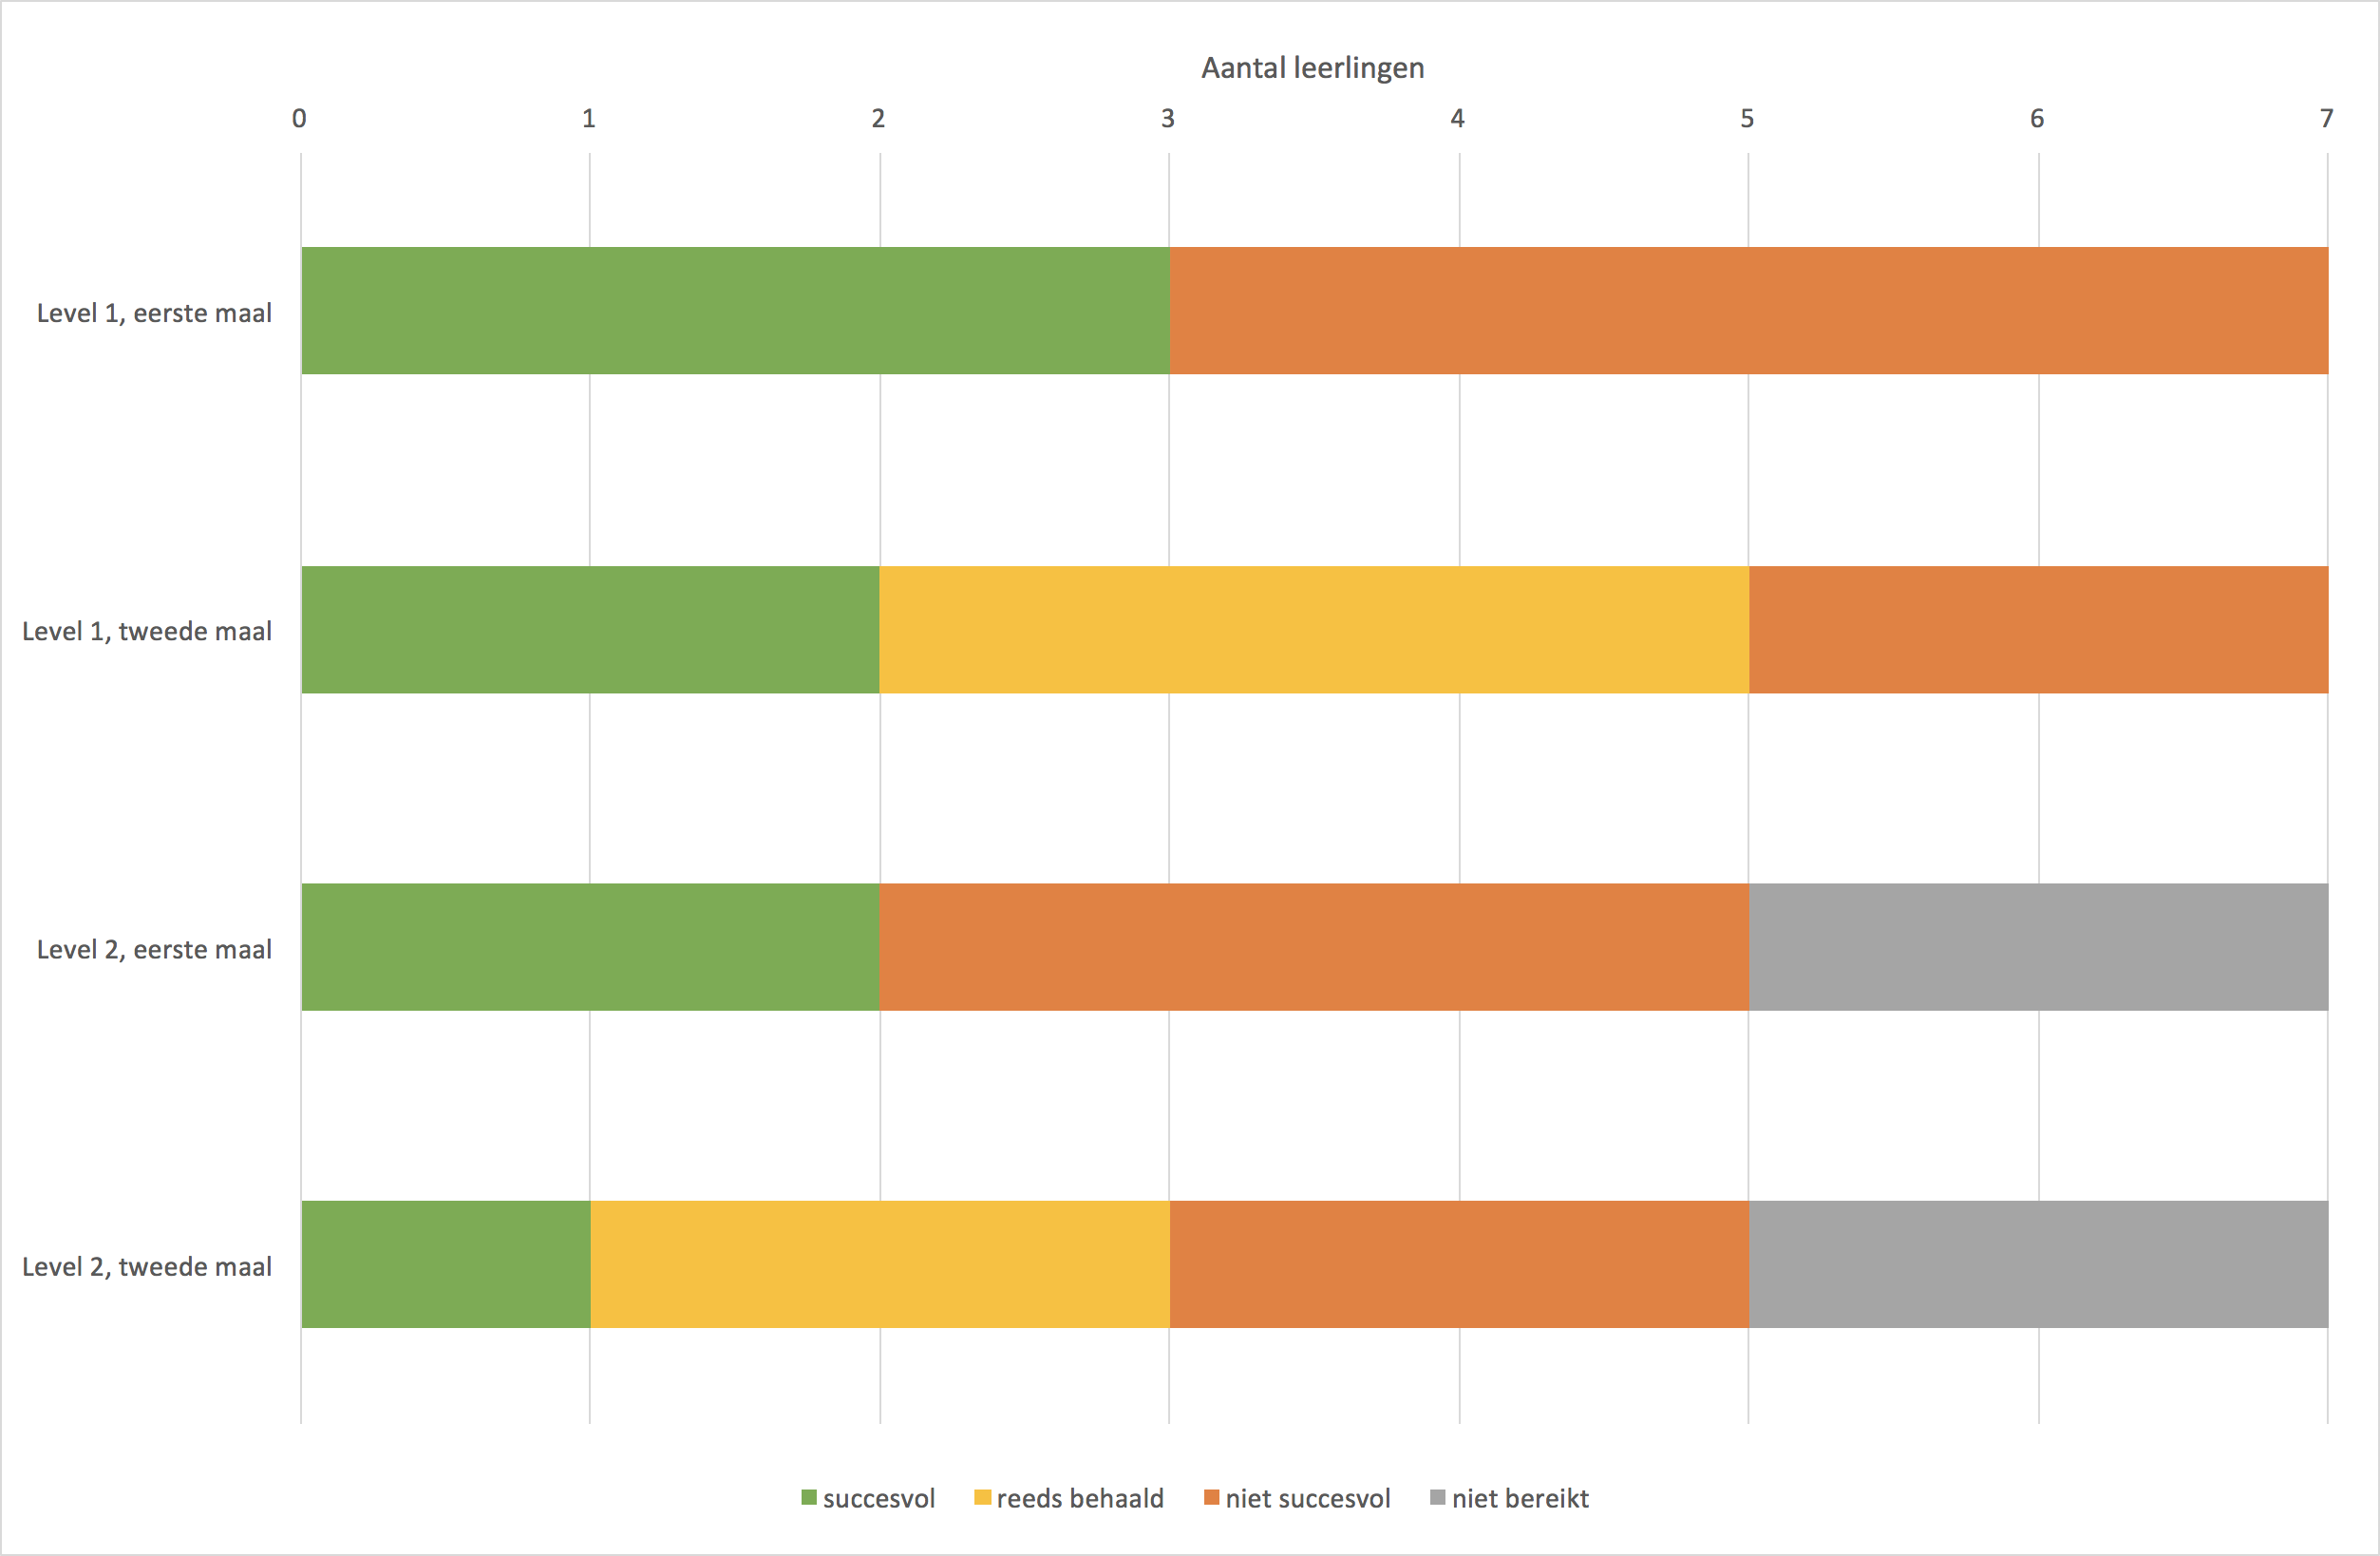
\includegraphics[width=\textwidth]{pictures/derde_iteratie.png}
        \caption{Resultaten gebruikersstudie derde iteratie}
        \label{figuur1}
   	\end{sidewaysfigure}
    
		\subsubsection{Enqu\^ete bij de leerlingen}
Tijdens de gebruikersstudies in de tweede en de derde iteratie werd er aan de leerlingen gevraagd om een aantal spelletjes te spelen van \textit{QuickMaths}. Nadat ze deze spelletjes gespeeld hadden, werd er hen gevraagd een korte enqu\^ete in te vullen. De resultaten van deze enqu\^ete en de evolutie tussen de twee iteraties heen worden in deze subsectie besproken.\\\\
De eerste vraag in de enqu\^ete ging over het gevoel van de leerling na het gebruik van de app. In Figuur~\ref{gebruik:app} worden de resultaten van deze vraag voorgesteld. In de tweede iteratie voelt $80\%$ van de deelnemers zich `goed' na het gebruik van de app. In de iteratie die erop volgt, voelt $67\%$ van de deelnemers zich `redelijk goed' tot `goed'.\\\\
De volgende vraag in de enqu\^ete polst naar de duidelijkheid van het spel dat in \textit{QuickMaths} gespeeld moet worden. Zoals in Figuur \ref{doel:spel} vastgesteld kan worden, vindt de meerderheid van de leerlingen het doel van het spel `duidelijk' tot `heel duidelijk'. Enkel in de derde iteratie zijn er twee leerlingen die het doel van het spel `onduidelijk' vonden.\\\\
E\'en van onze doelstellingen bij het ontwikkelen van \textit{QuickMaths} is dat je het spel kan spelen zonder veel instructies op voorhand te moeten krijgen. Daarvoor stelden we aan de leerlingen de vraag of de manier waarop je het spel moet spelen duidelijk was van in het begin. In Figuur~\ref{duidelijk:begin} kunnen we vaststellen dat het voor de leerlingen toch niet altijd duidelijk was hoe ze het spel moesten spelen. Dit probleem werd opgelost door het toevoegen van een kleine tutorial die aan de speler toont waar je precies moet klikken in de applicatie.\\\\
Met \textit{QuickMaths} willen we bereiken dat de leerlingen van de eerste graad middelbare school op regelmatige basis het hoofdrekenen in wiskunde oefenen. Daarom stelden wij de vraag hoe vaak de leerlingen de app zouden willen gebruiken. Zoals we in Figuur~\ref{aantal:spelen} kunnen vaststellen, zijn de leerlingen gemotiveerd om de app van meerdere keren per maand tot meerdere keren per week te gebruiken.\\\\
Een volgende vraag polste naar de moeilijkheid van het \textit{QuickMaths}-spel. De leerlingen kregen de opdracht om de app een score te geven tussen $1$ en $10$, wat respectievelijk `heel gemakkelijk' en `heel moeilijk' voorstelt. De resultaten van deze vraag staan voorgesteld in Figuur~\ref{moeilijkheid}.
In de tweede iteratie gaven de leerlingen gemiddeld een score van $4.8$ voor de moeilijkheid van het spel. De mediaan is er $5.0$.
In de derde iteratie gaven de leerlingen gemiddeld een score van $3.5$ voor de moeilijkheid van het spel. De mediaan is er $3.0$.
We kunnen hier vaststellen dat de leerlingen tussen de twee iteraties door het spel gemakkelijker vonden dankzij de aanpassingen die doorgevoerd werden in de applicatie. Zo werd onder andere de balk waar de antwoorden aangeduid moeten worden een rij naar boven geschoven. Dit maakte het spel eenvoudiger voor de leerlingen.\\\\
In de derde iteratie voegden we achtergrond- en spelgeluiden toe aan \textit{QuickMaths}. Ook hier wilden wij van de leerlingen weten wat hun gevoel was bij deze geluiden. Bij de achtergrondmuziek (Figuur~\ref{achtergrondmuziek}) kunnen we concluderen dat het merendeel van de studenten deze muziek `motiverend' vinden. Slechts \'e\'en leerling van de zes vond deze muziek `storend'. Bij de spelgeluiden (Figuur~\ref{spelgeluiden}) kunnen we geen conclusies maken. Het merendeel van de studenten heeft geen mening over de spelgeluiden, de andere opties zijn evenredig verdeeld.

\begin{figure}
	\centering
    \begin{subfigure}[b]{0.48\textwidth}
        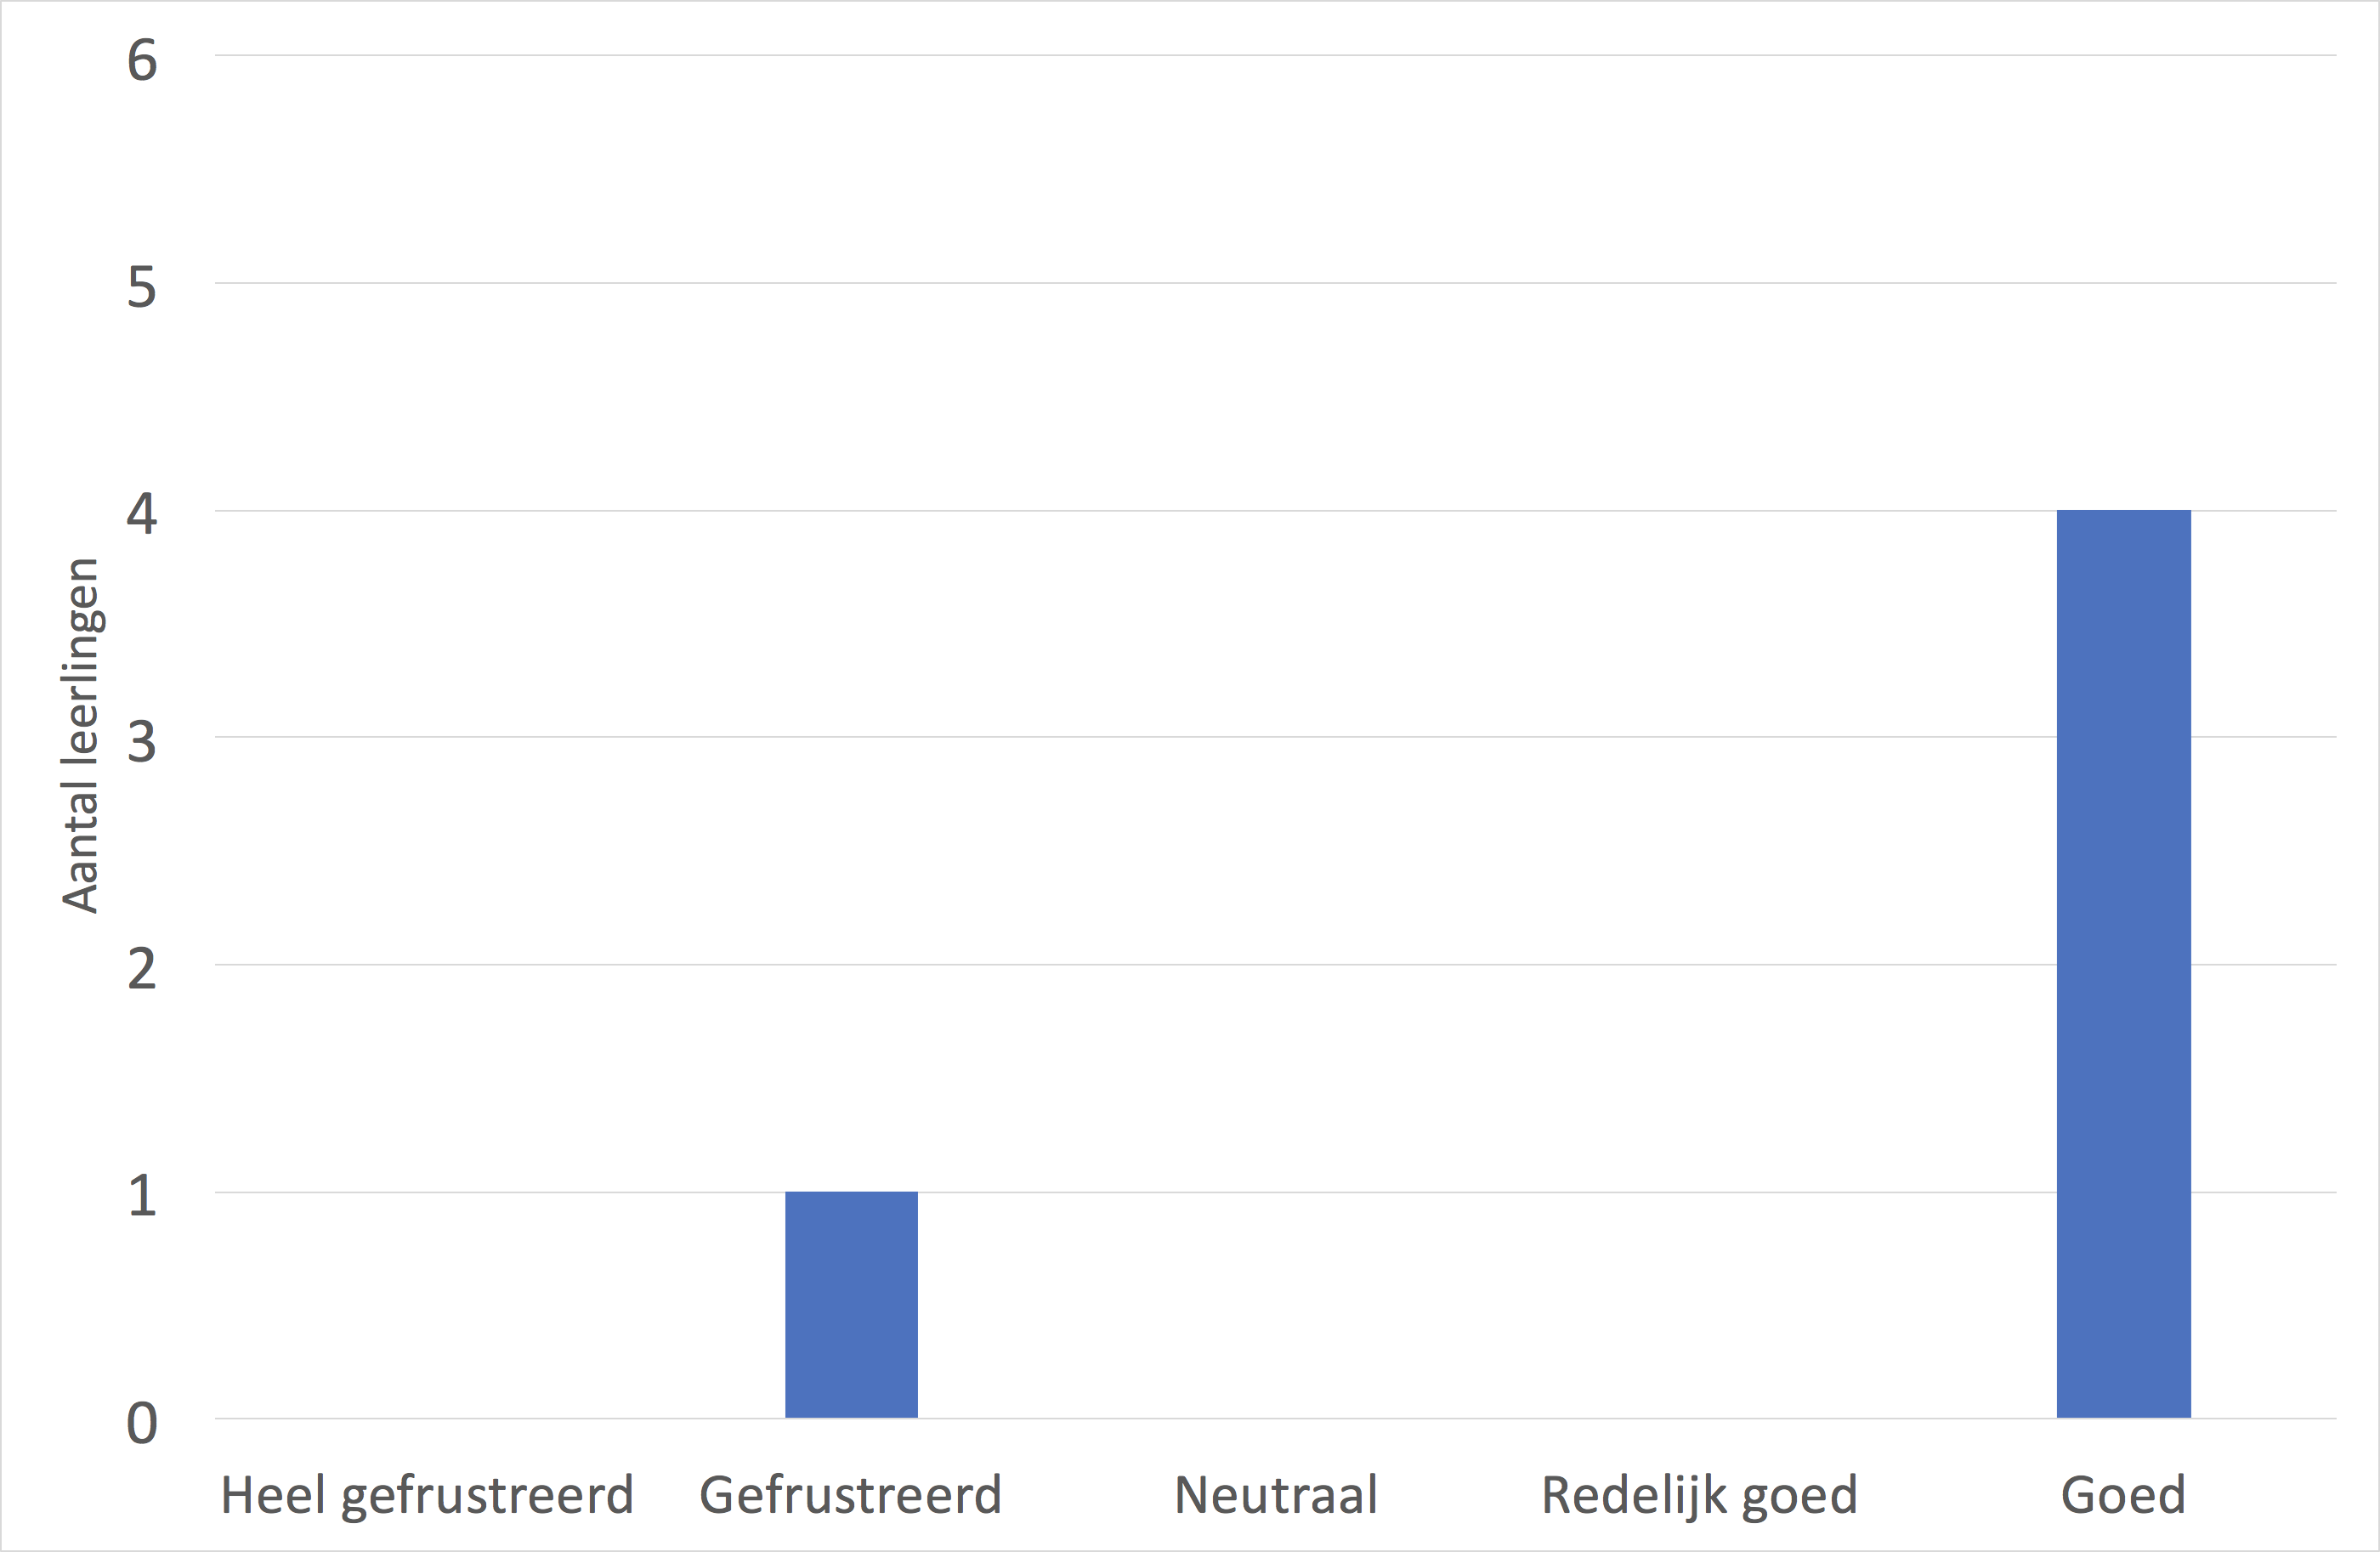
\includegraphics[width=\textwidth]{pictures/2_GebruikApp.png}
        \caption{tweede iteratie}
        \label{gebruik:app:twee}
    \end{subfigure}
    ~
    \begin{subfigure}[b]{0.48\textwidth}
        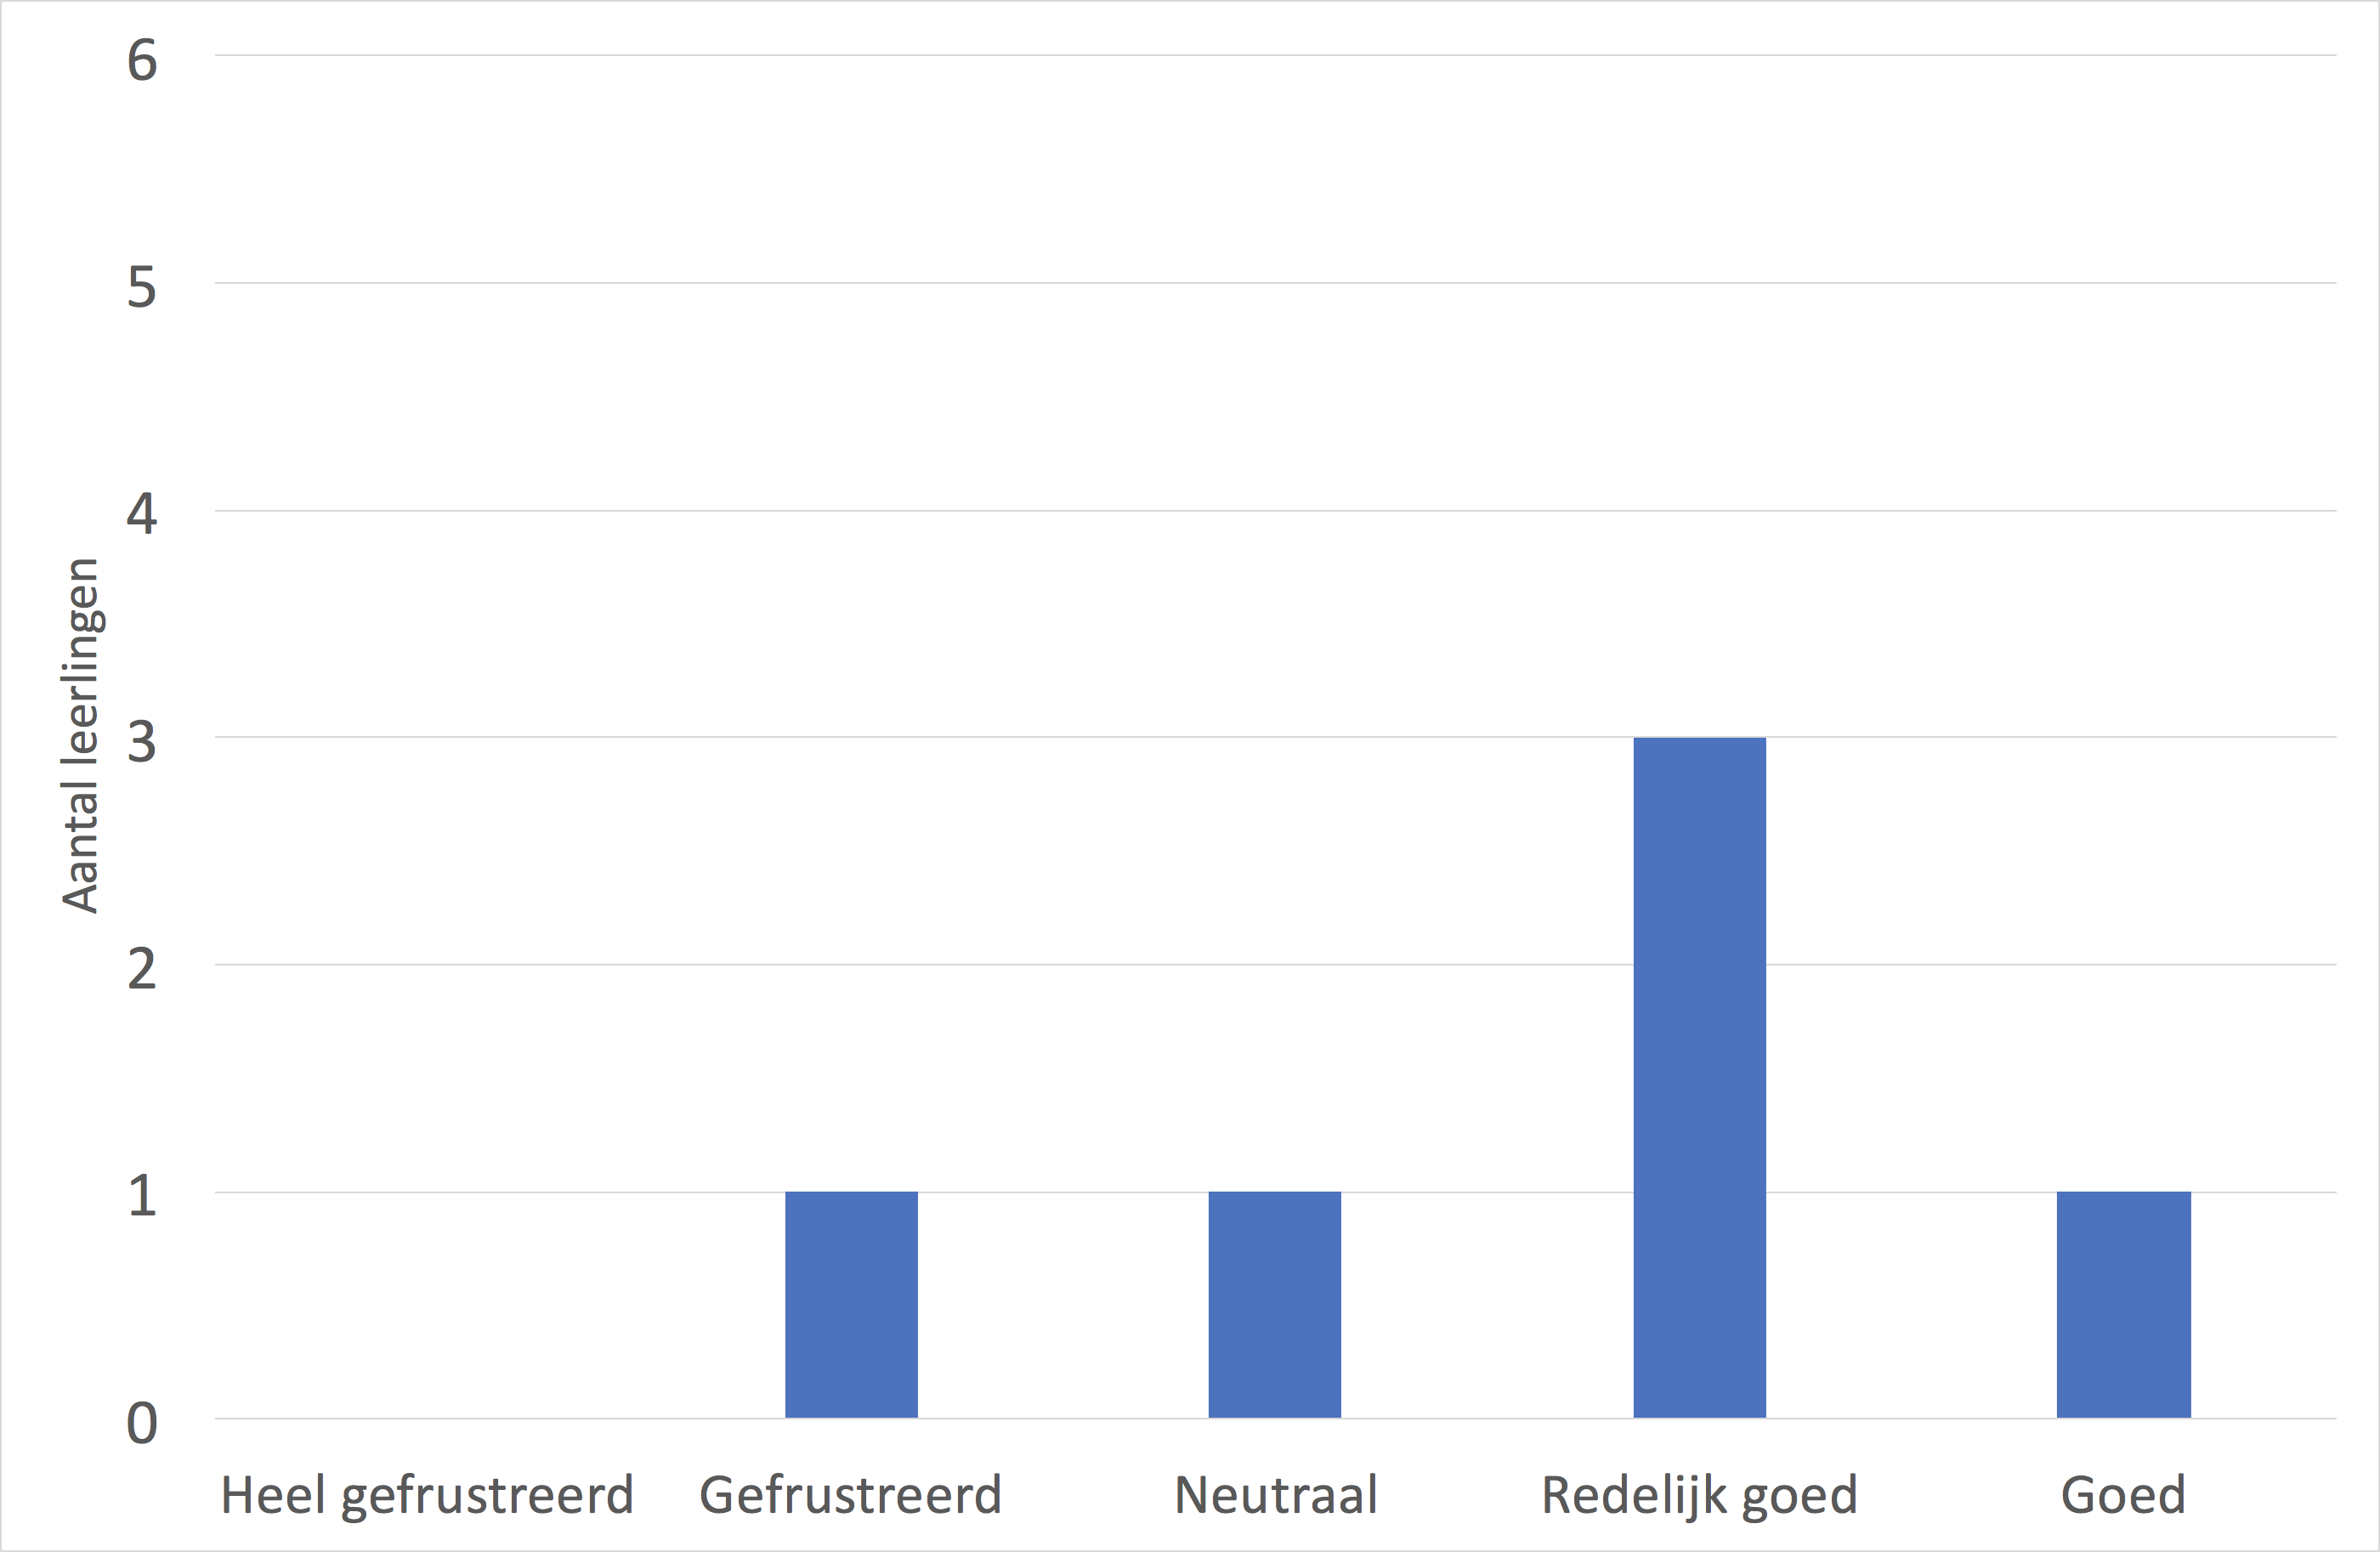
\includegraphics[width=\textwidth]{pictures/3_GebruikApp.png}
        \caption{derde iteratie}
        \label{gebruik:app:drie}
    \end{subfigure}
    \caption{Hoe voel je jezelf na het gebruik van de app?}\label{gebruik:app}
\end{figure}

\begin{figure}
	\centering
    \begin{subfigure}[b]{0.48\textwidth}
        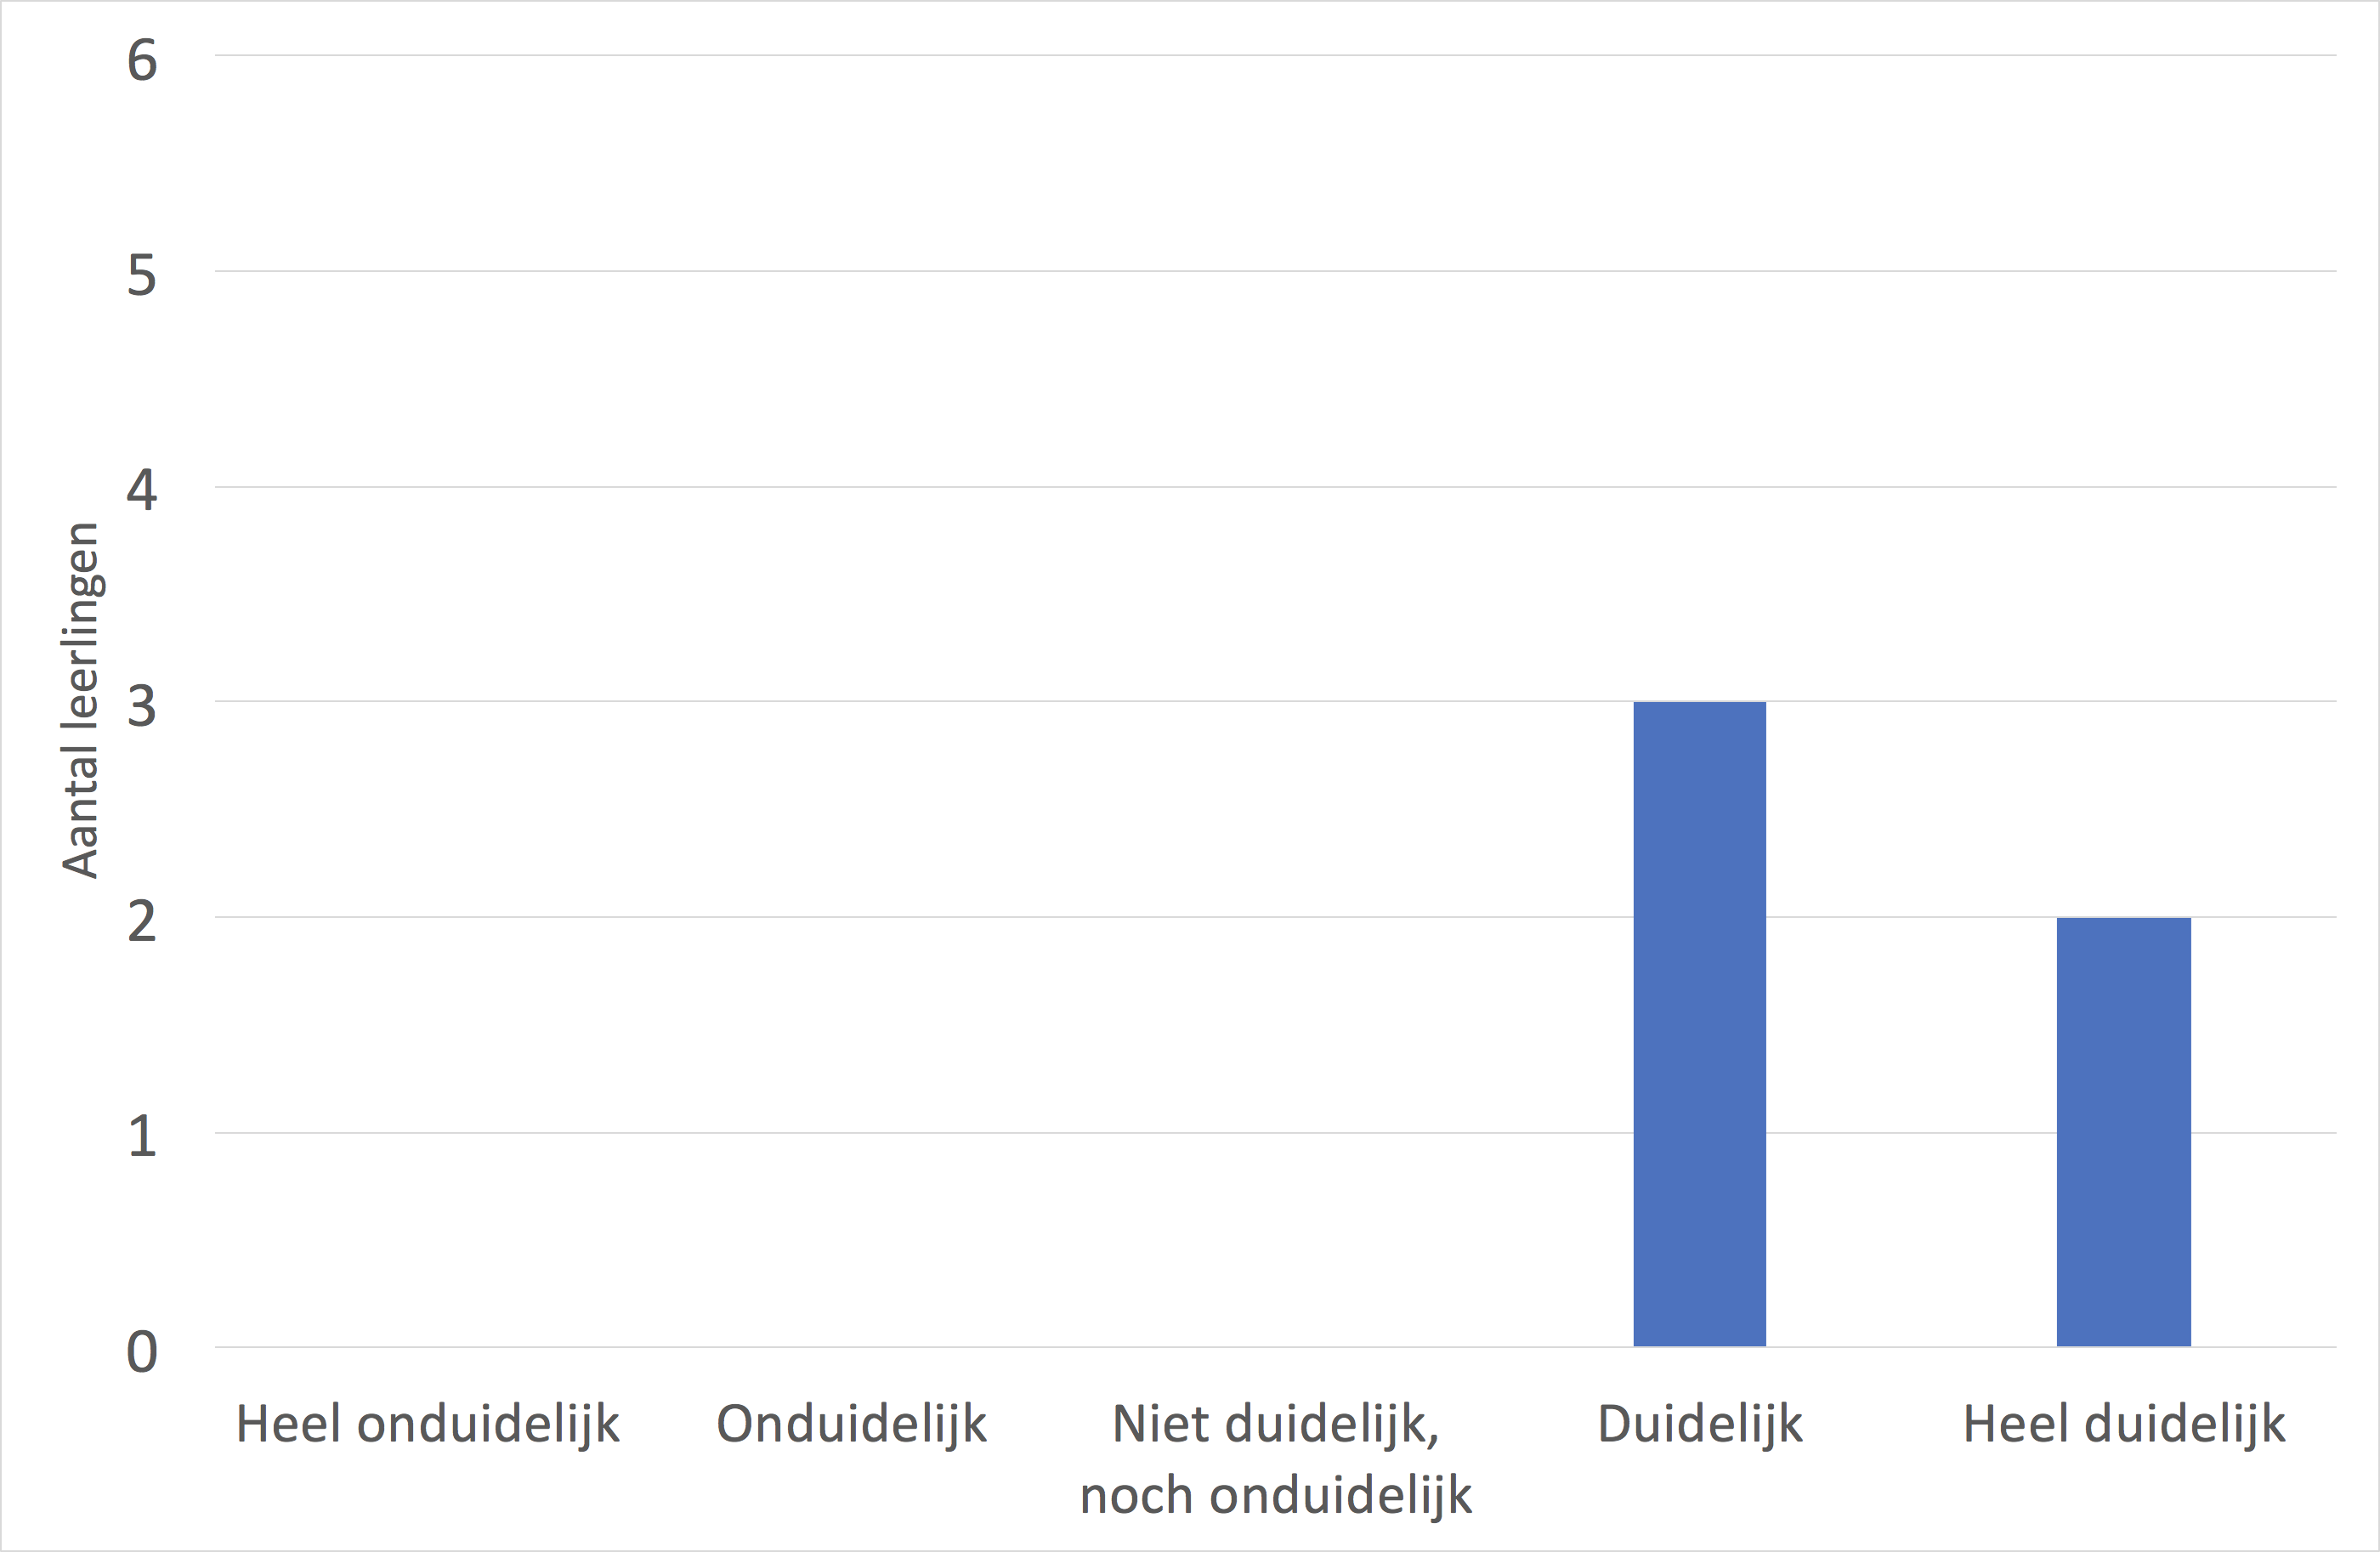
\includegraphics[width=\textwidth]{pictures/2_DoelSpel.png}
        \caption{tweede iteratie}
        \label{doel:spel:twee}
    \end{subfigure}
    ~
    \begin{subfigure}[b]{0.48\textwidth}
        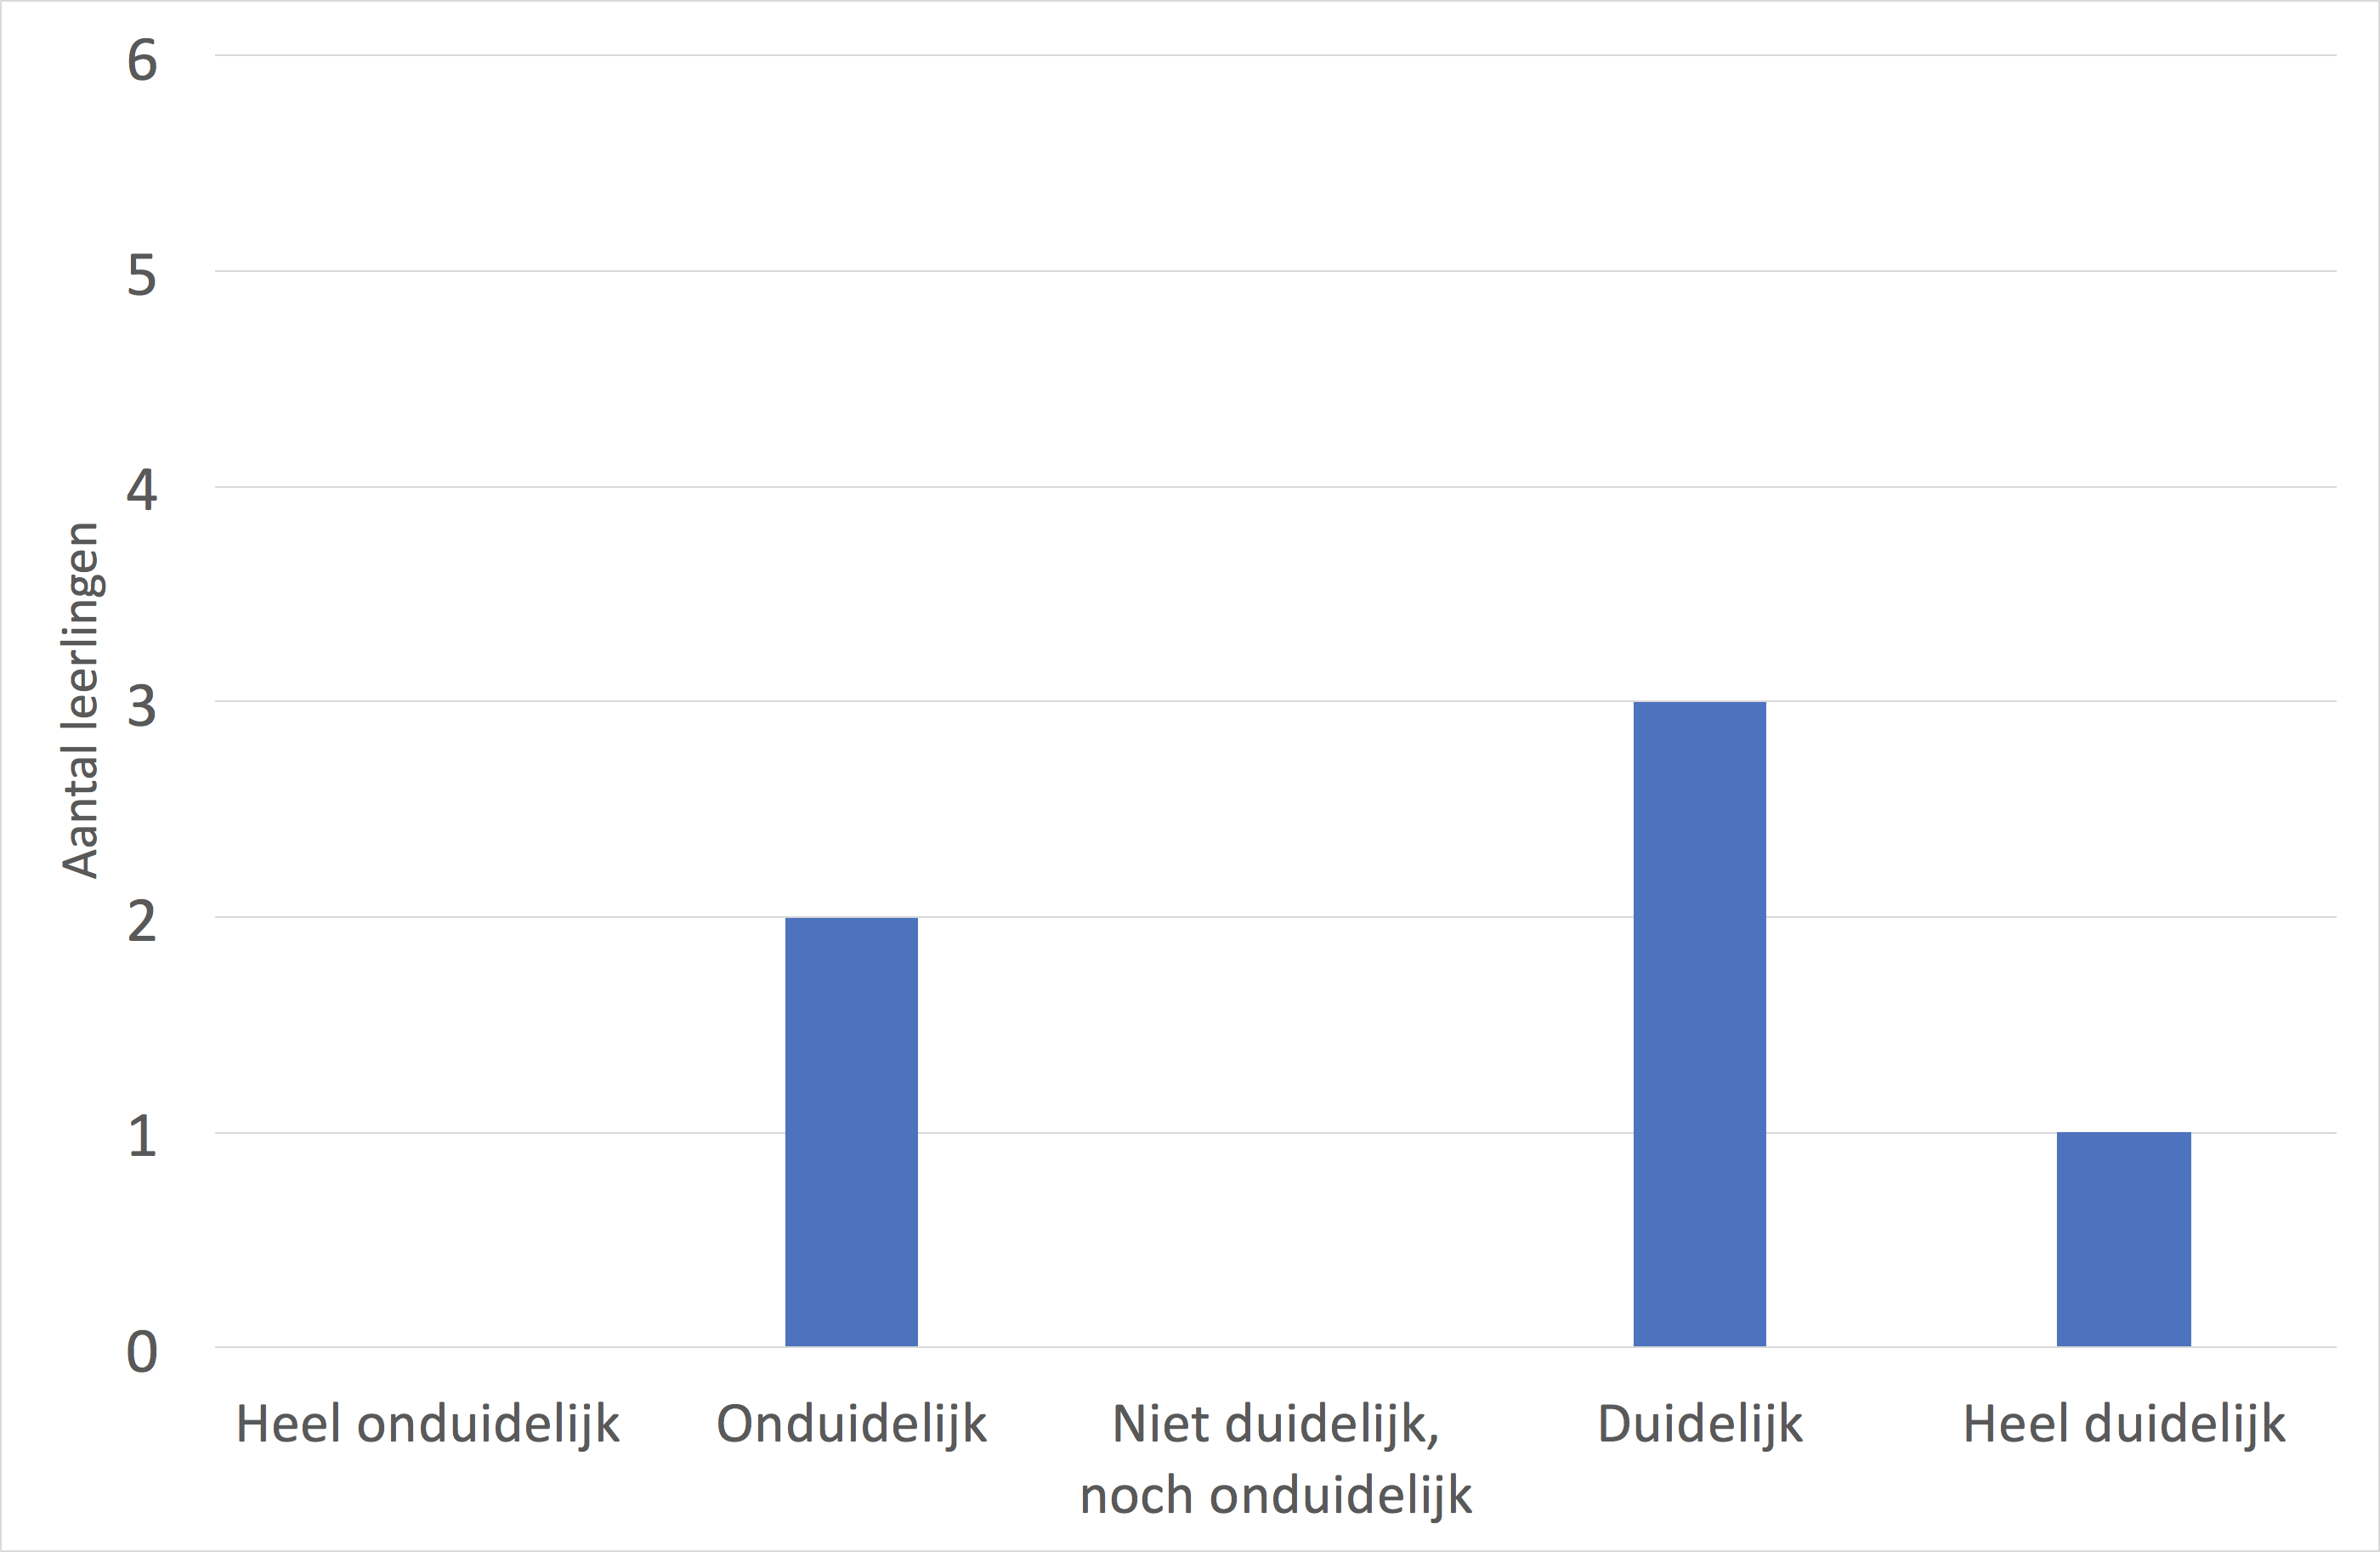
\includegraphics[width=\textwidth]{pictures/3_DoelSpel.png}
        \caption{derde iteratie}
        \label{doel:spel:drie}
    \end{subfigure}
    \caption{Hoe duidelijk was het doel van het spel?}\label{doel:spel}
\end{figure}

\begin{figure}
	\centering
    \begin{subfigure}[b]{0.48\textwidth}
        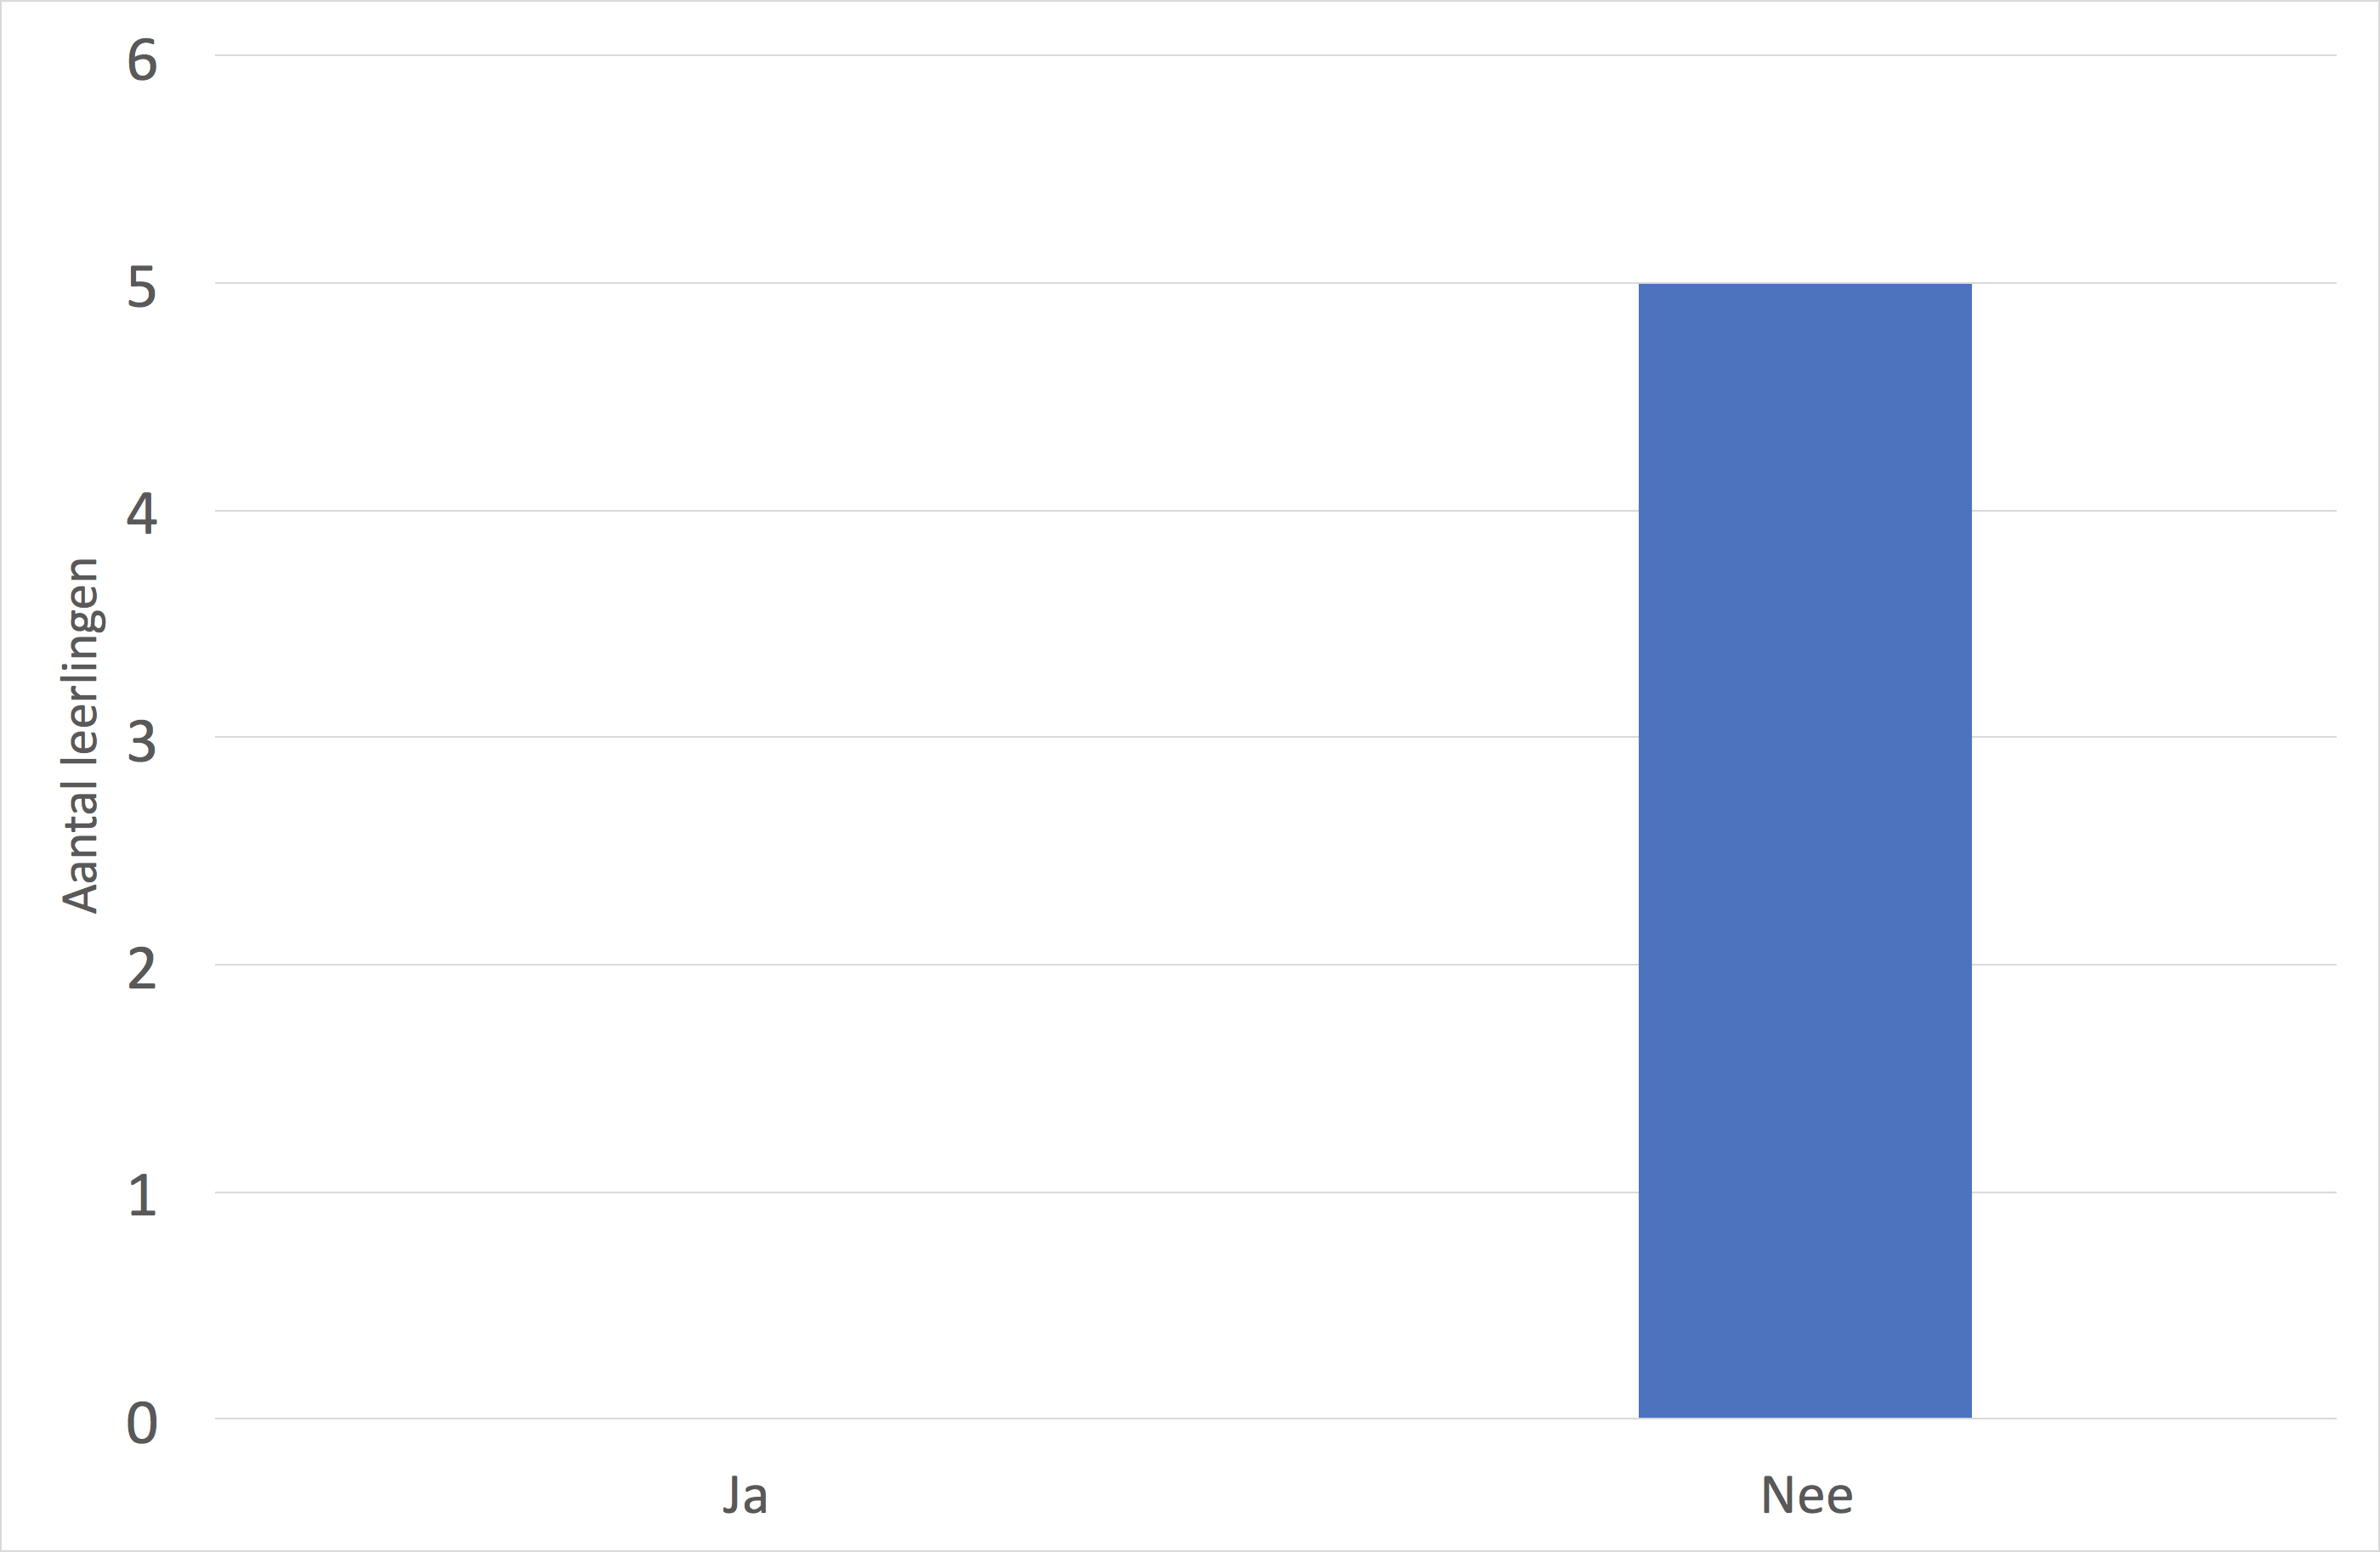
\includegraphics[width=\textwidth]{pictures/2_DuidelijkBegin.png}
        \caption{tweede iteratie}
        \label{duidelijk:begin:twee}
    \end{subfigure}
    ~
    \begin{subfigure}[b]{0.48\textwidth}
        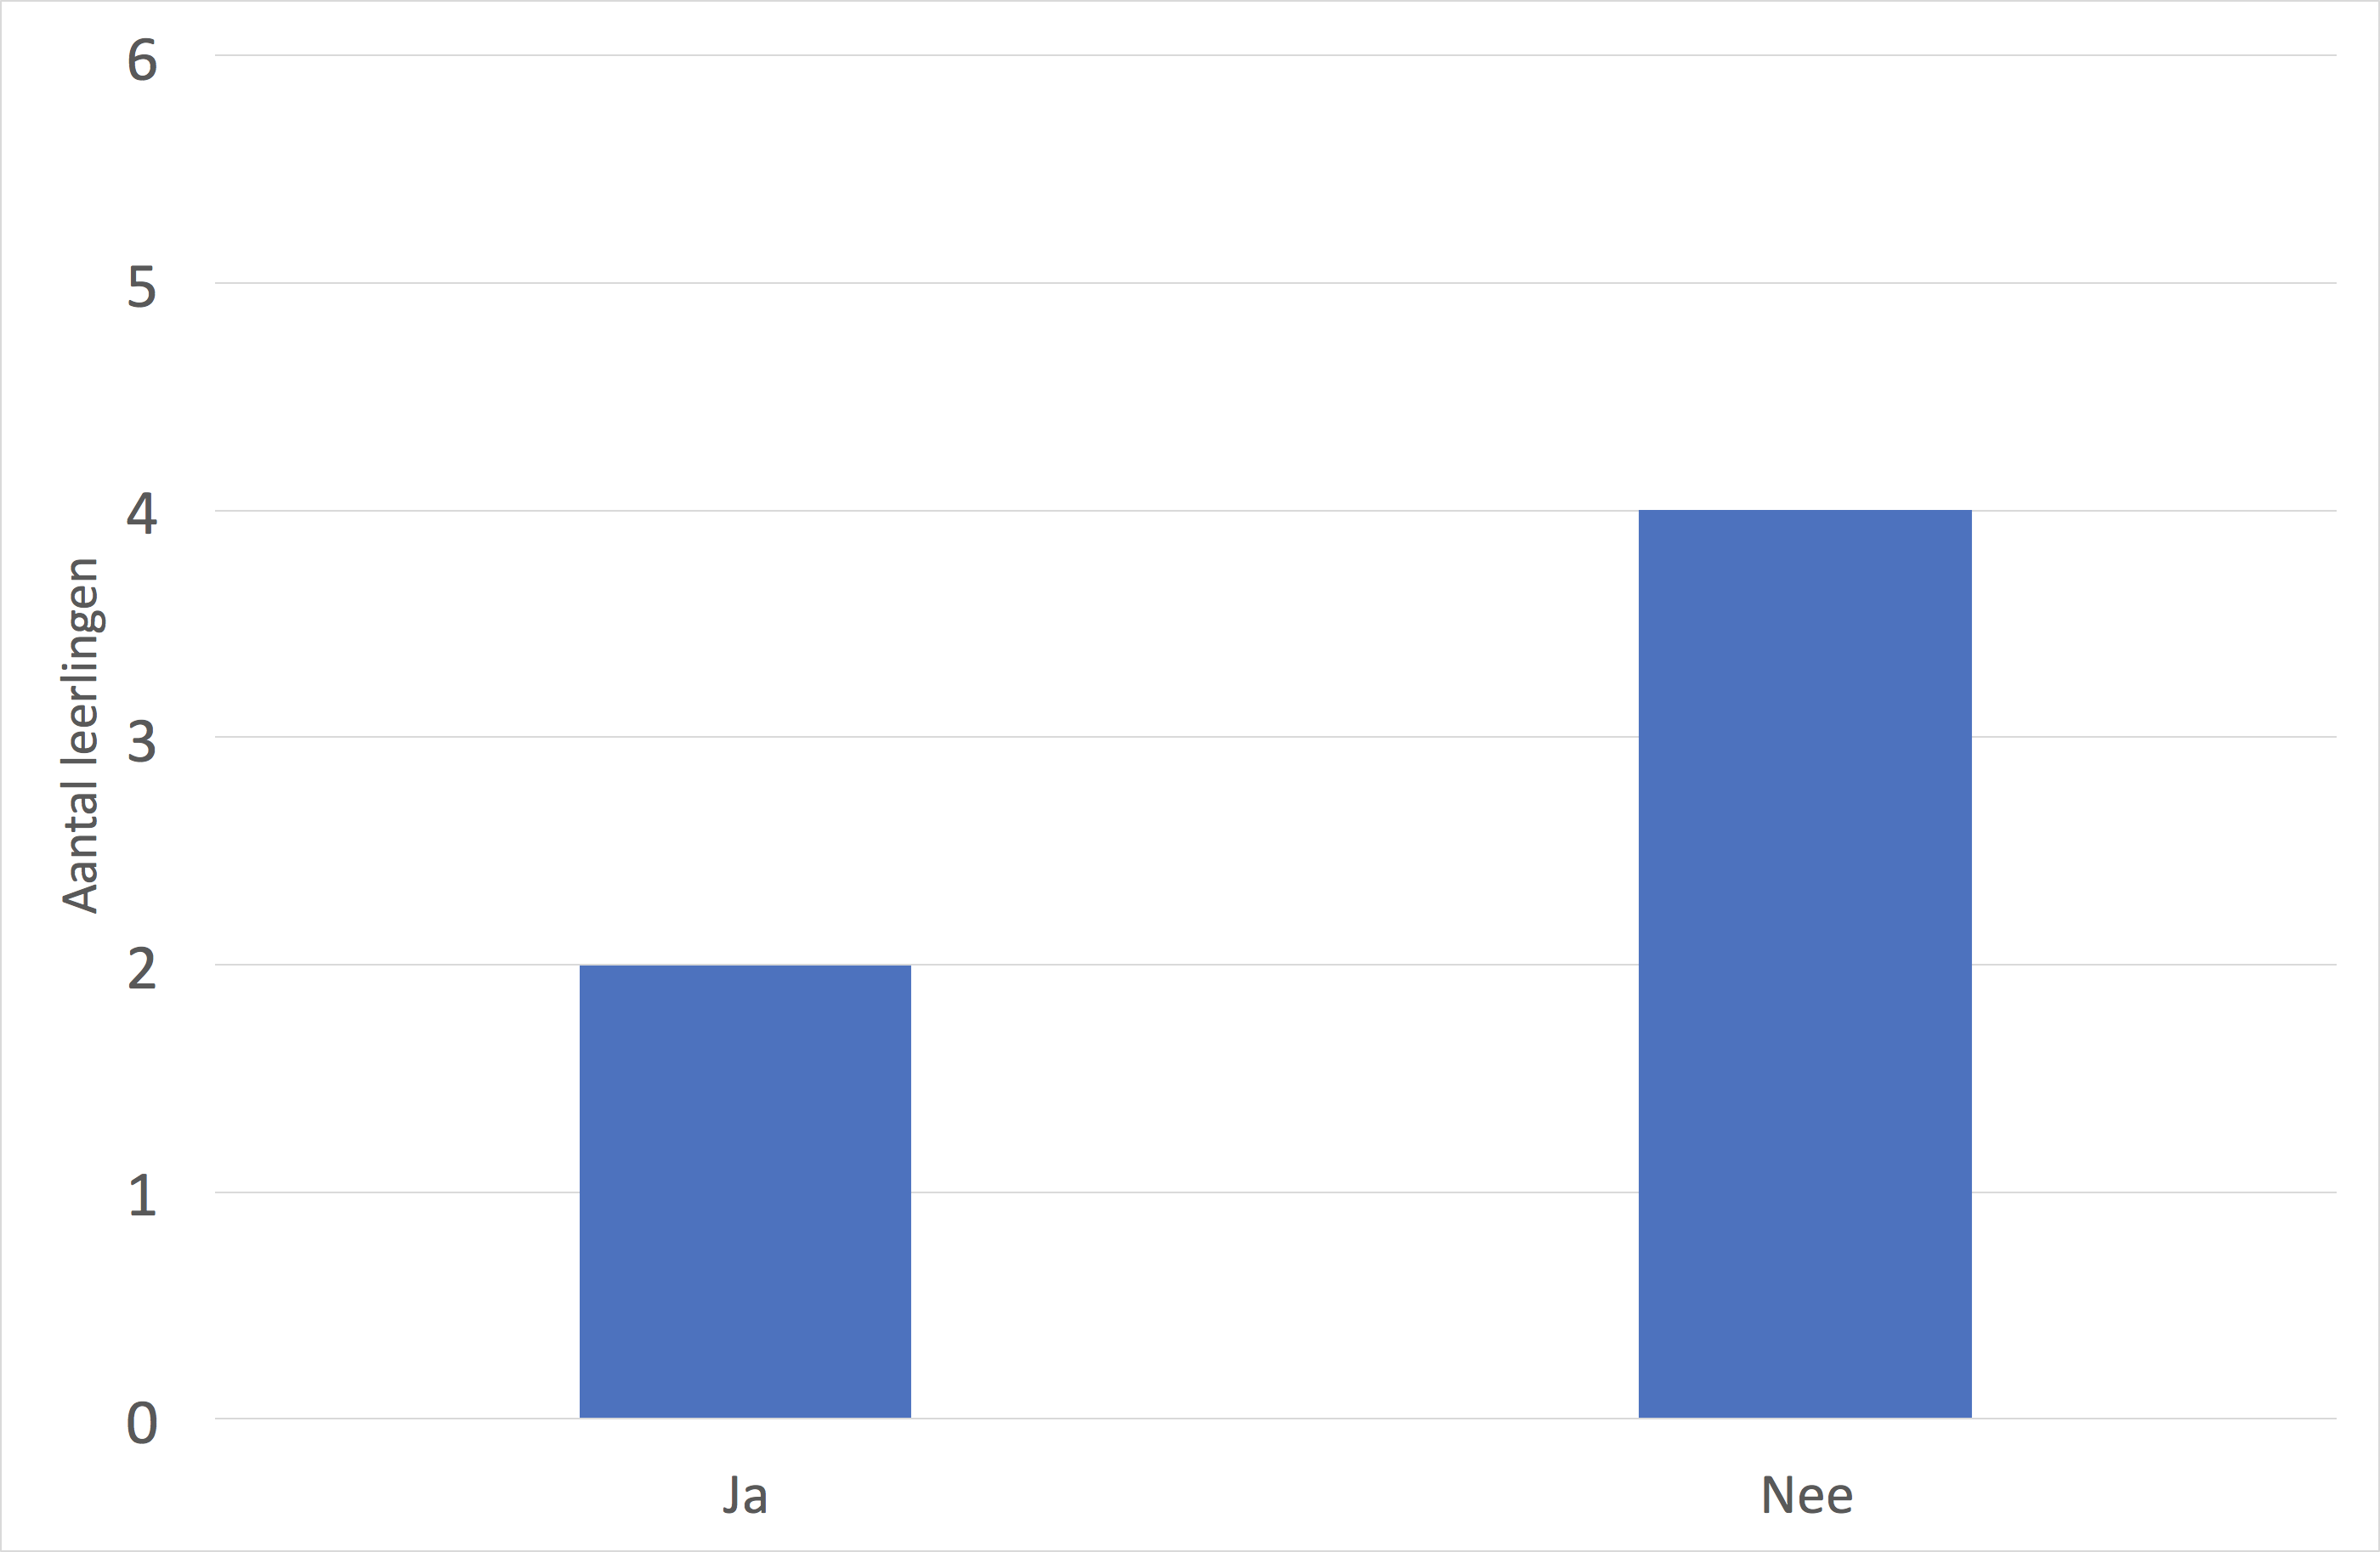
\includegraphics[width=\textwidth]{pictures/3_DuidelijkBegin.png}
        \caption{derde iteratie}
        \label{duidelijk:begin:drie}
    \end{subfigure}
    \caption{Was de manier waarop je moet spelen vanaf het begin duidelijk?}\label{duidelijk:begin}
\end{figure}

\begin{figure}
	\centering
    \begin{subfigure}[b]{0.48\textwidth}
        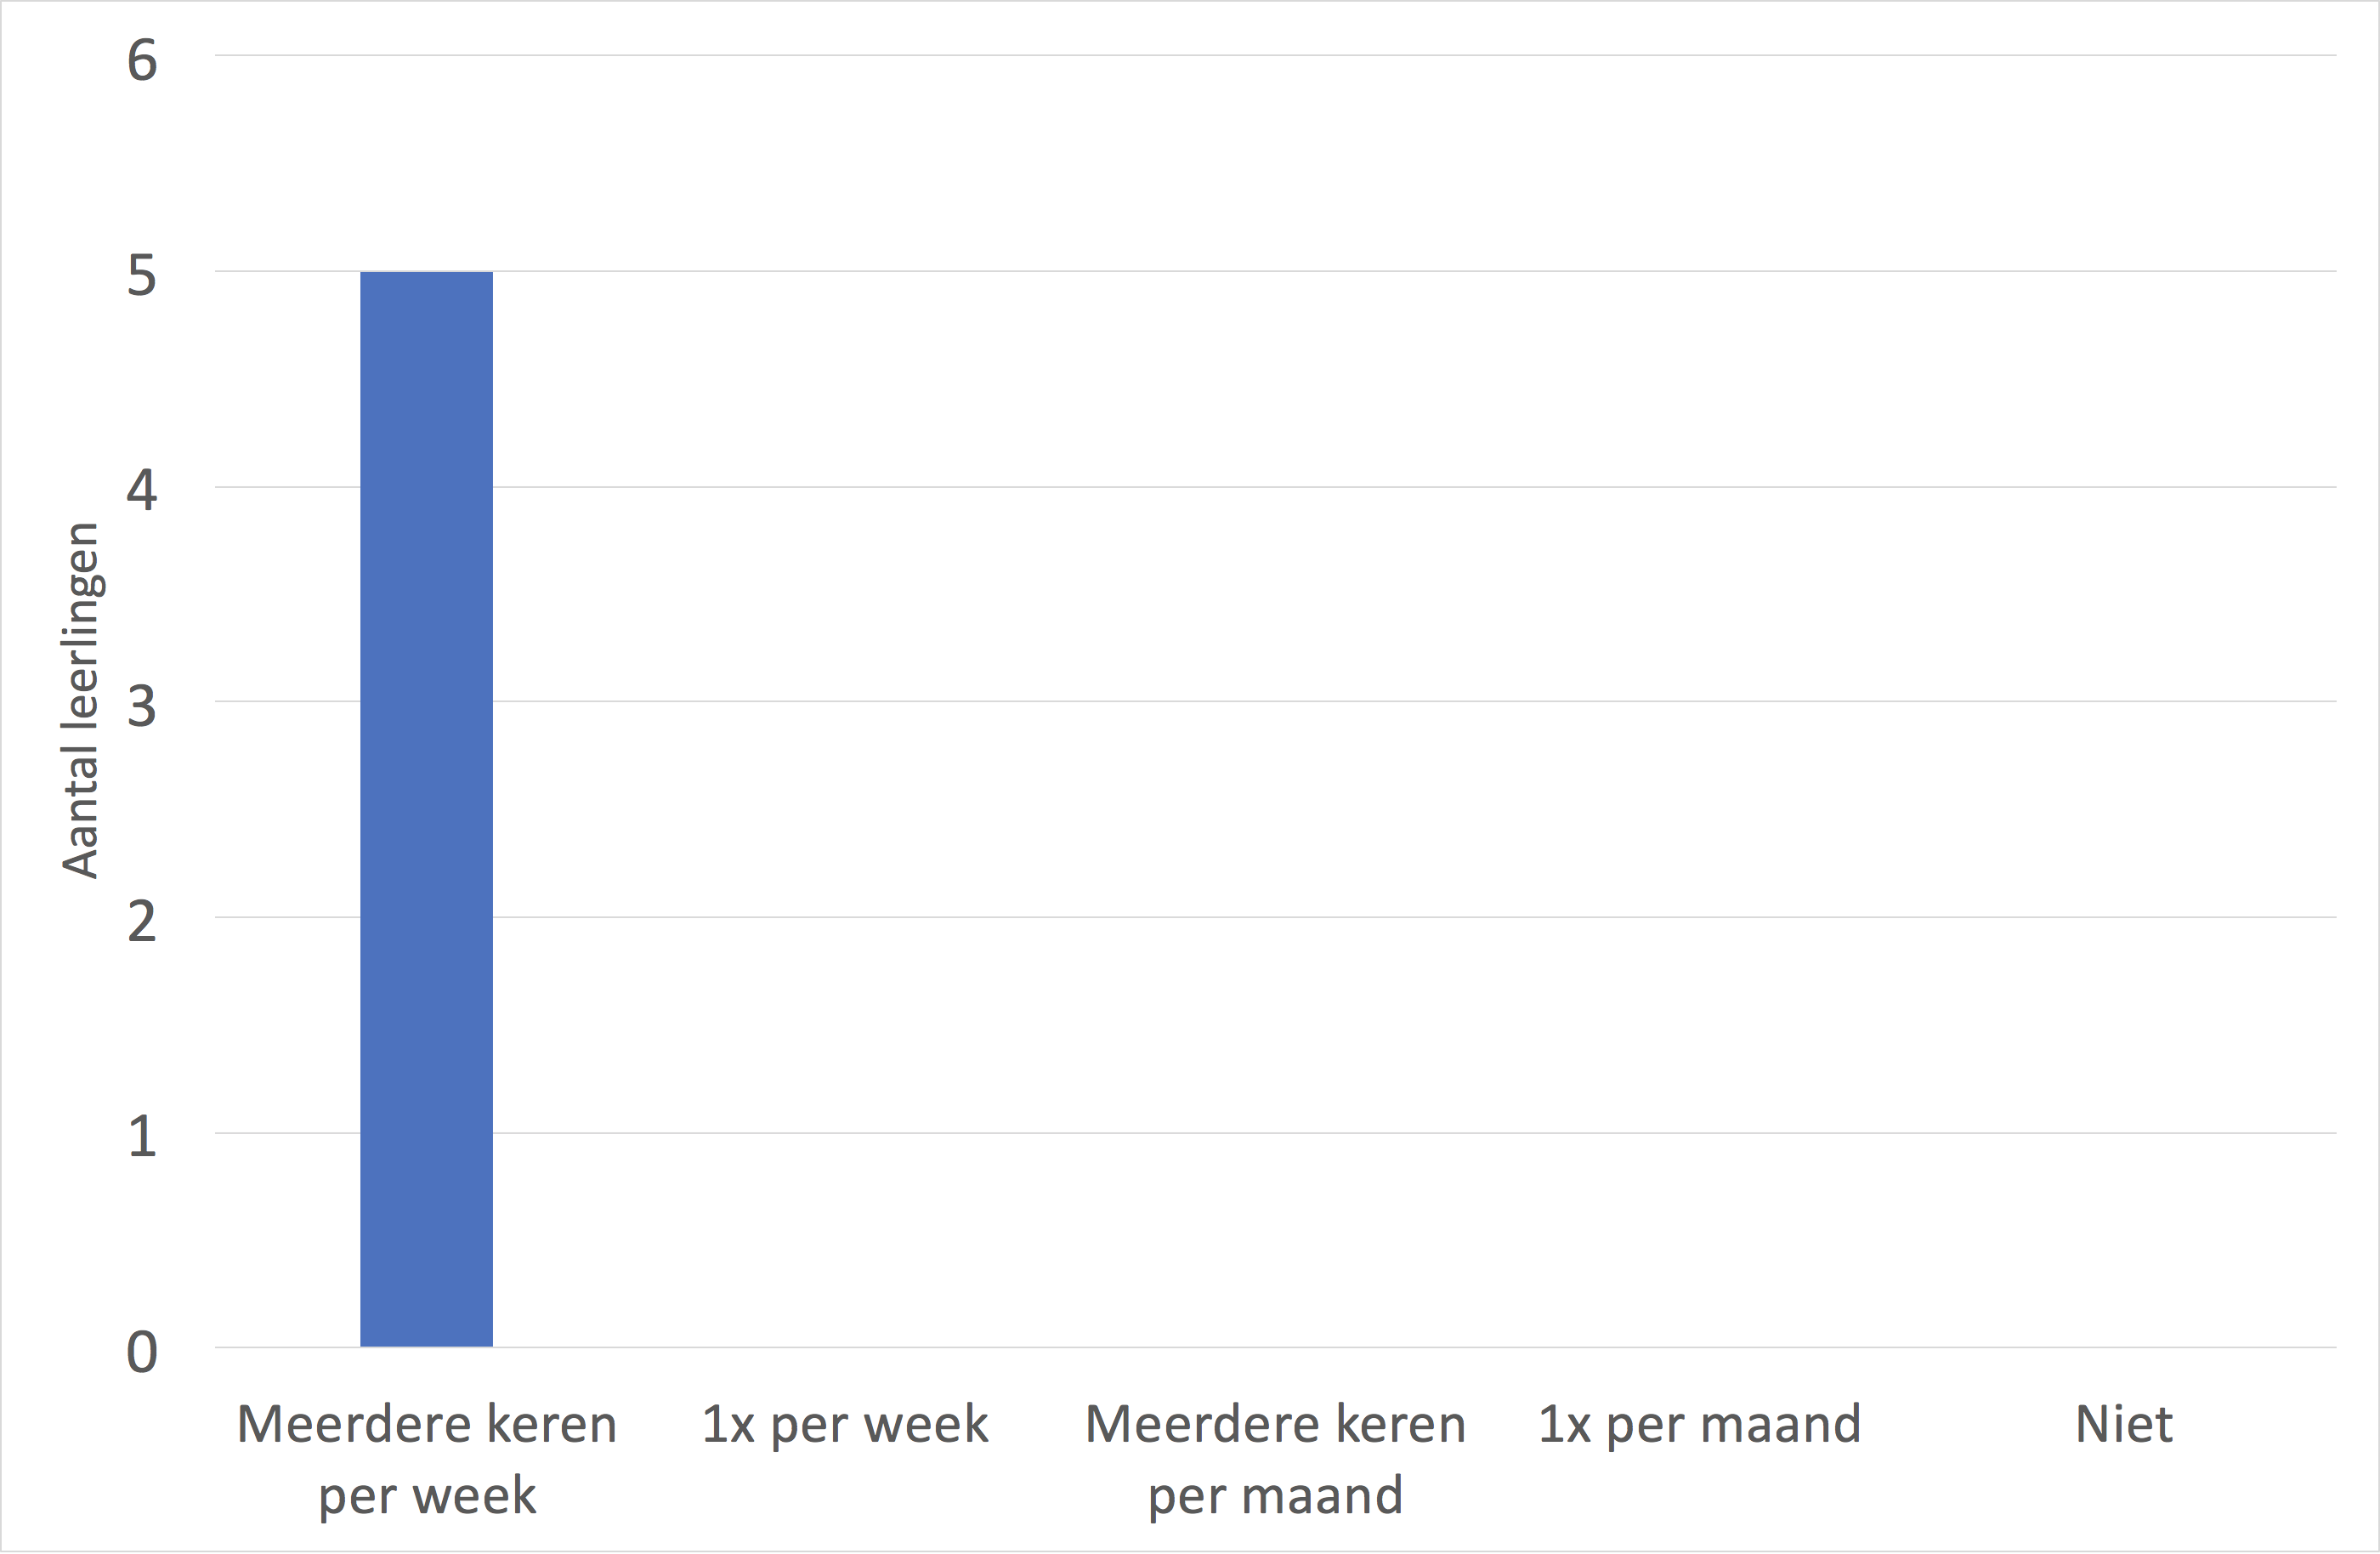
\includegraphics[width=\textwidth]{pictures/2_AantalSpelen.png}
        \caption{tweede iteratie}
        \label{aantal:spelen:twee}
    \end{subfigure}
    ~
    \begin{subfigure}[b]{0.48\textwidth}
        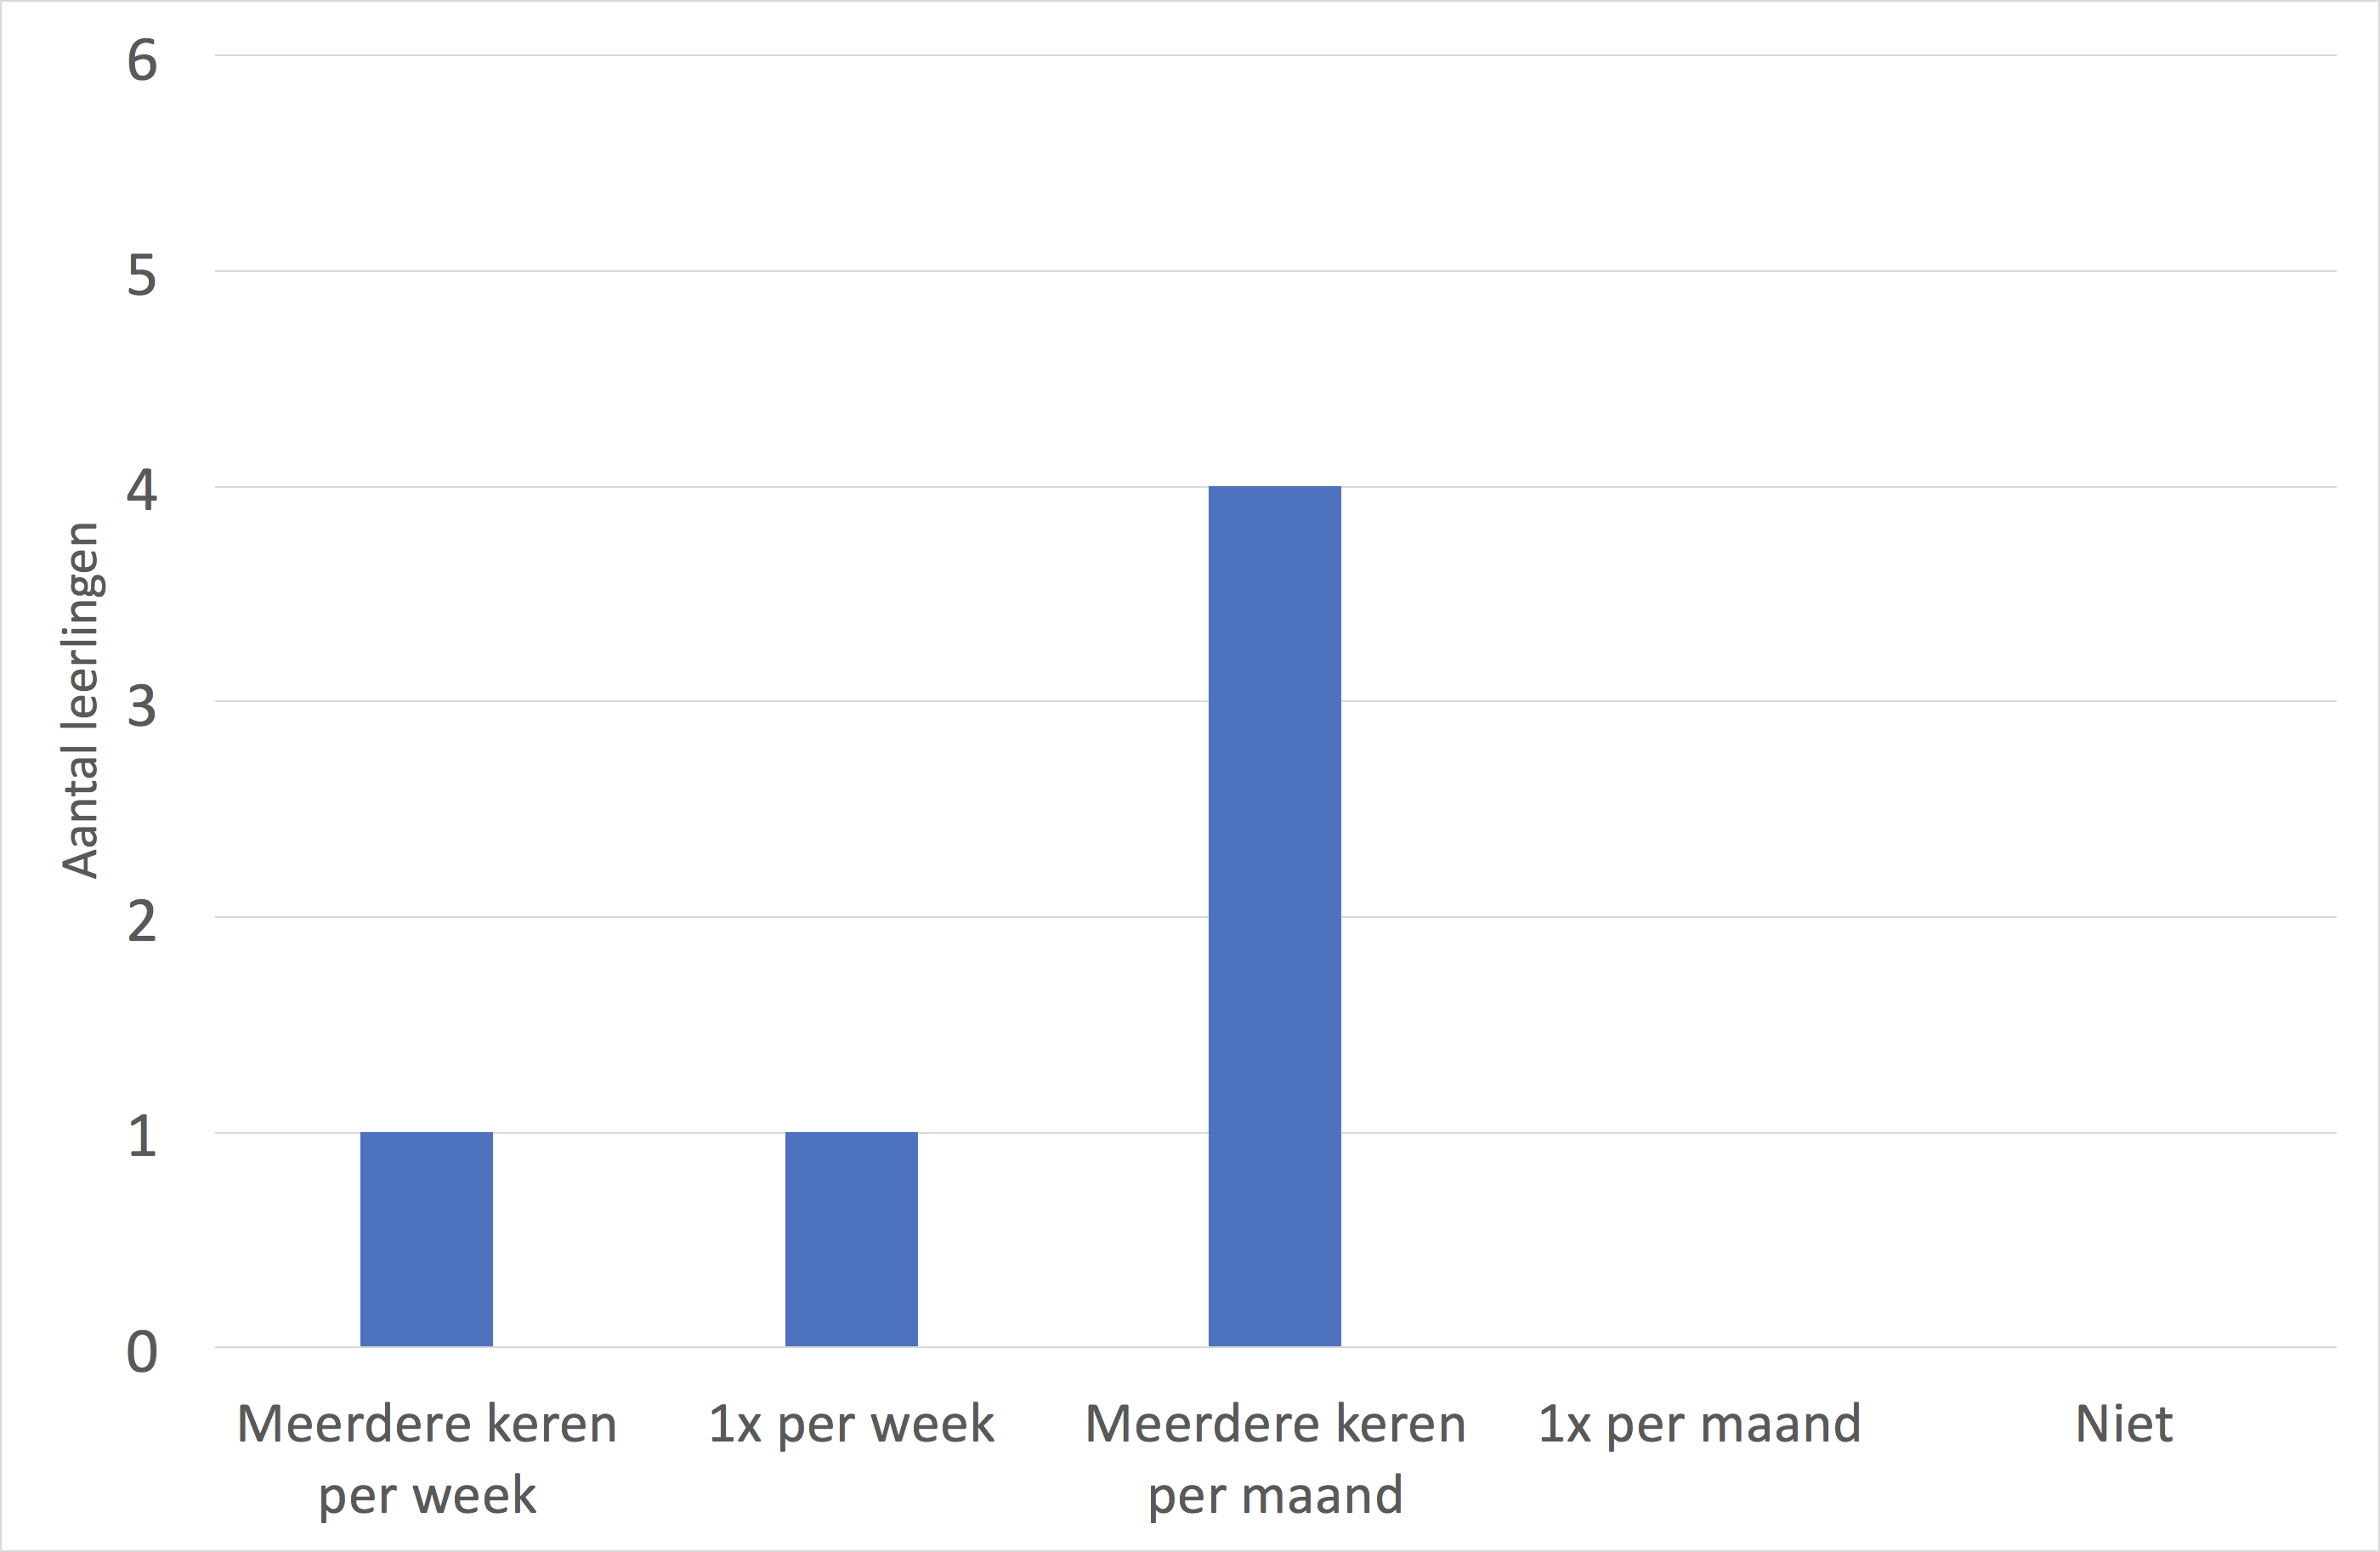
\includegraphics[width=\textwidth]{pictures/3_AantalSpelen.png}
        \caption{derde iteratie}
        \label{aantal:spelen:drie}
    \end{subfigure}
    \caption{Hoe vaak zou je het spel willen spelen?}\label{aantal:spelen}
\end{figure}

\begin{figure}
	\centering
    \begin{subfigure}[b]{0.48\textwidth}
        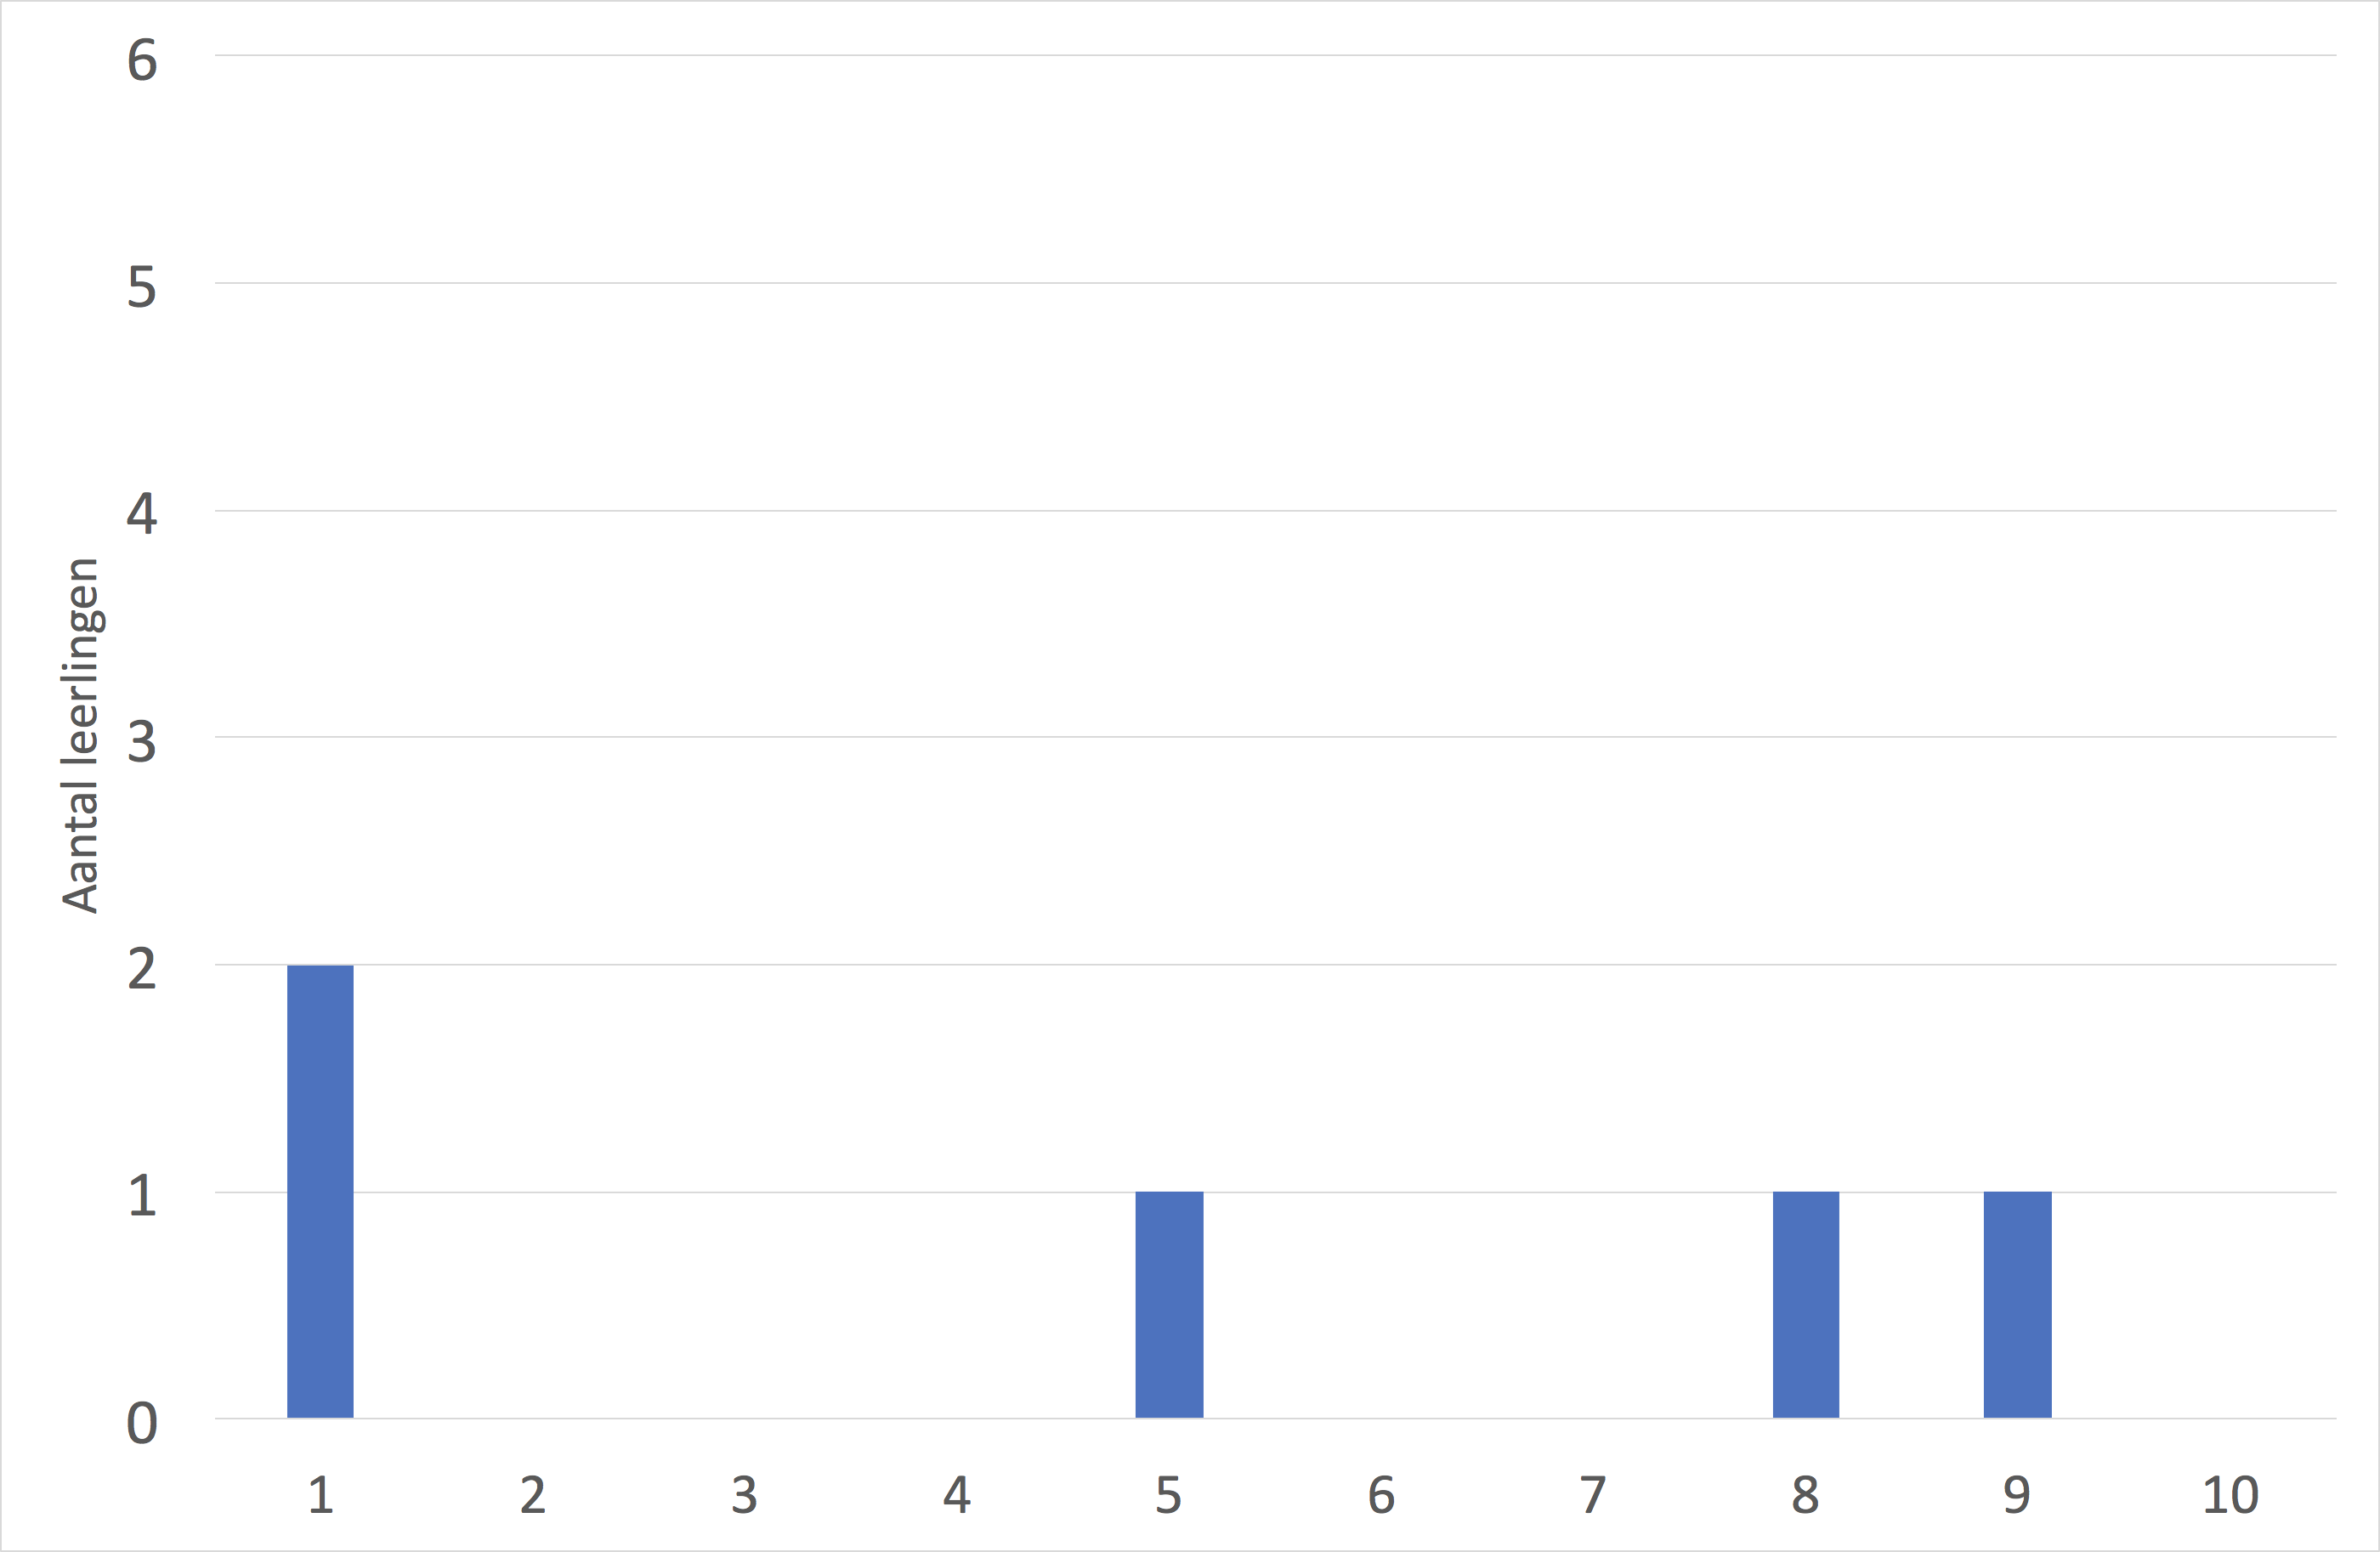
\includegraphics[width=\textwidth]{pictures/2_Moeilijkheid.png}
        \caption{tweede iteratie}
        \label{moeilijkheid:twee}
    \end{subfigure}
    ~
    \begin{subfigure}[b]{0.48\textwidth}
        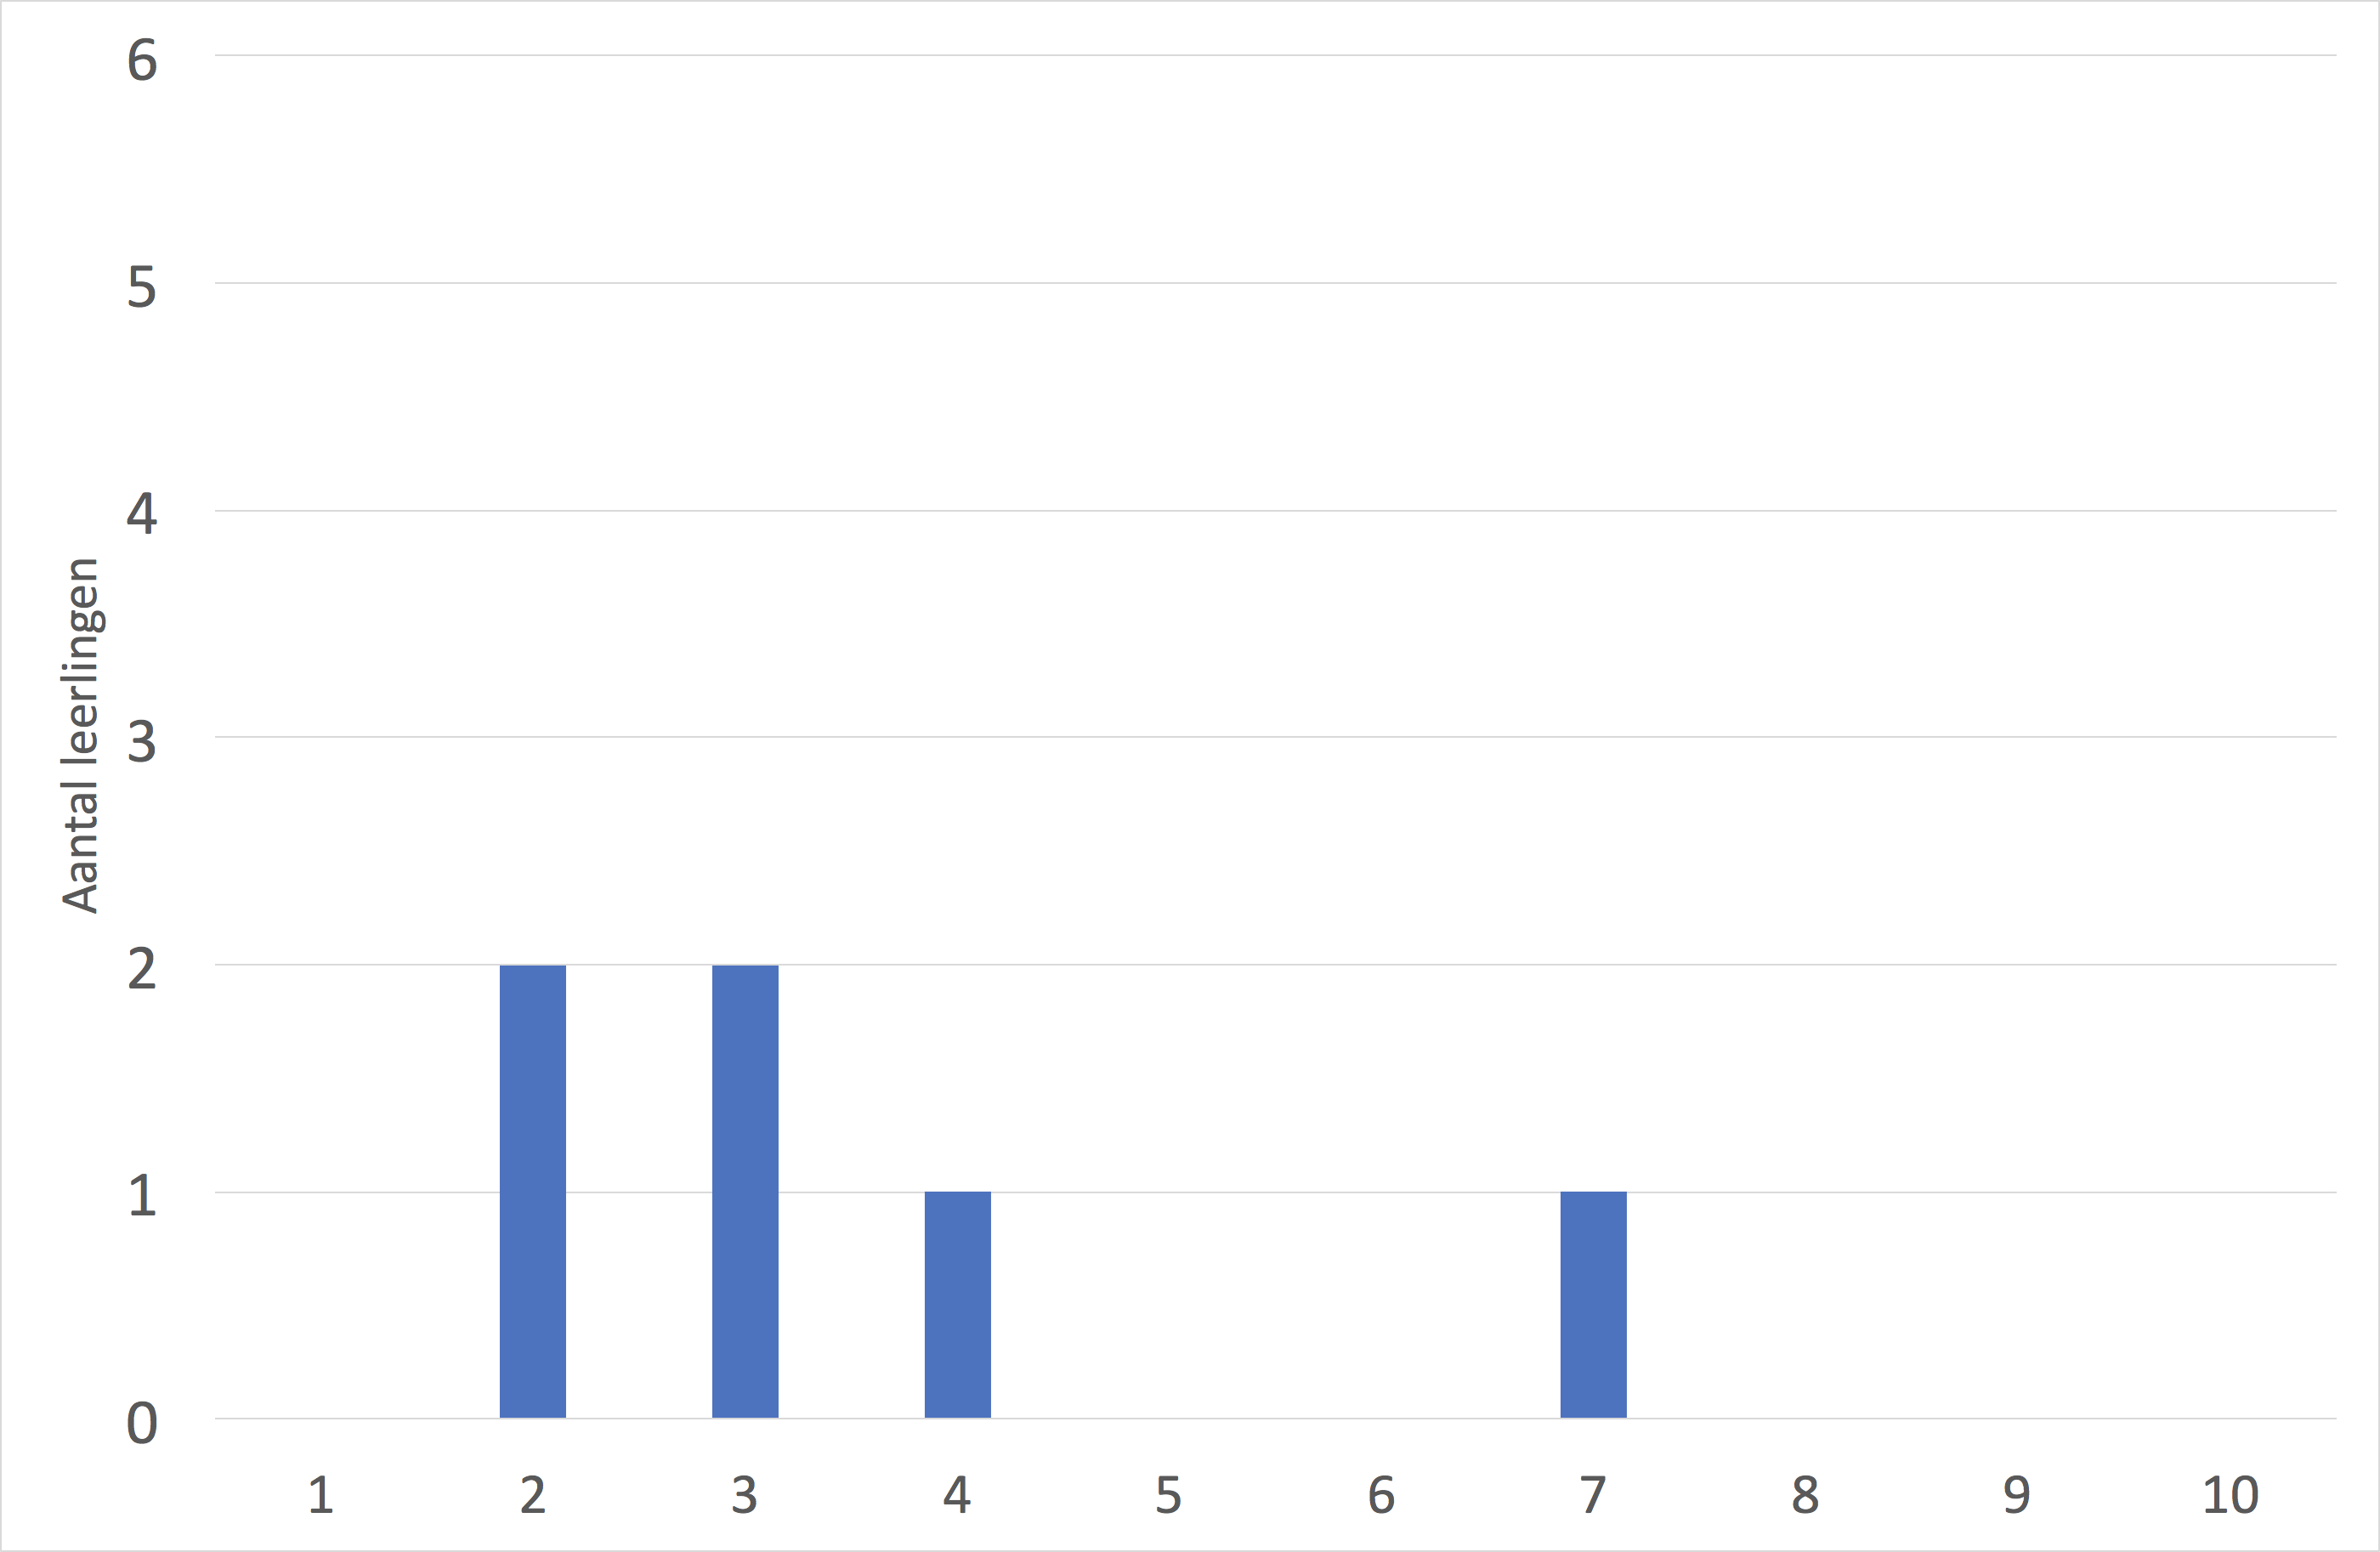
\includegraphics[width=\textwidth]{pictures/3_Moeilijkheid.png}
        \caption{derde iteratie}
        \label{moeilijkheid:drie}
    \end{subfigure}
    \caption{Wat vond je van de moeilijkheid van het spel?}\label{moeilijkheid}
\end{figure}

\begin{figure}
	\centering
    \begin{subfigure}[b]{0.48\textwidth}
        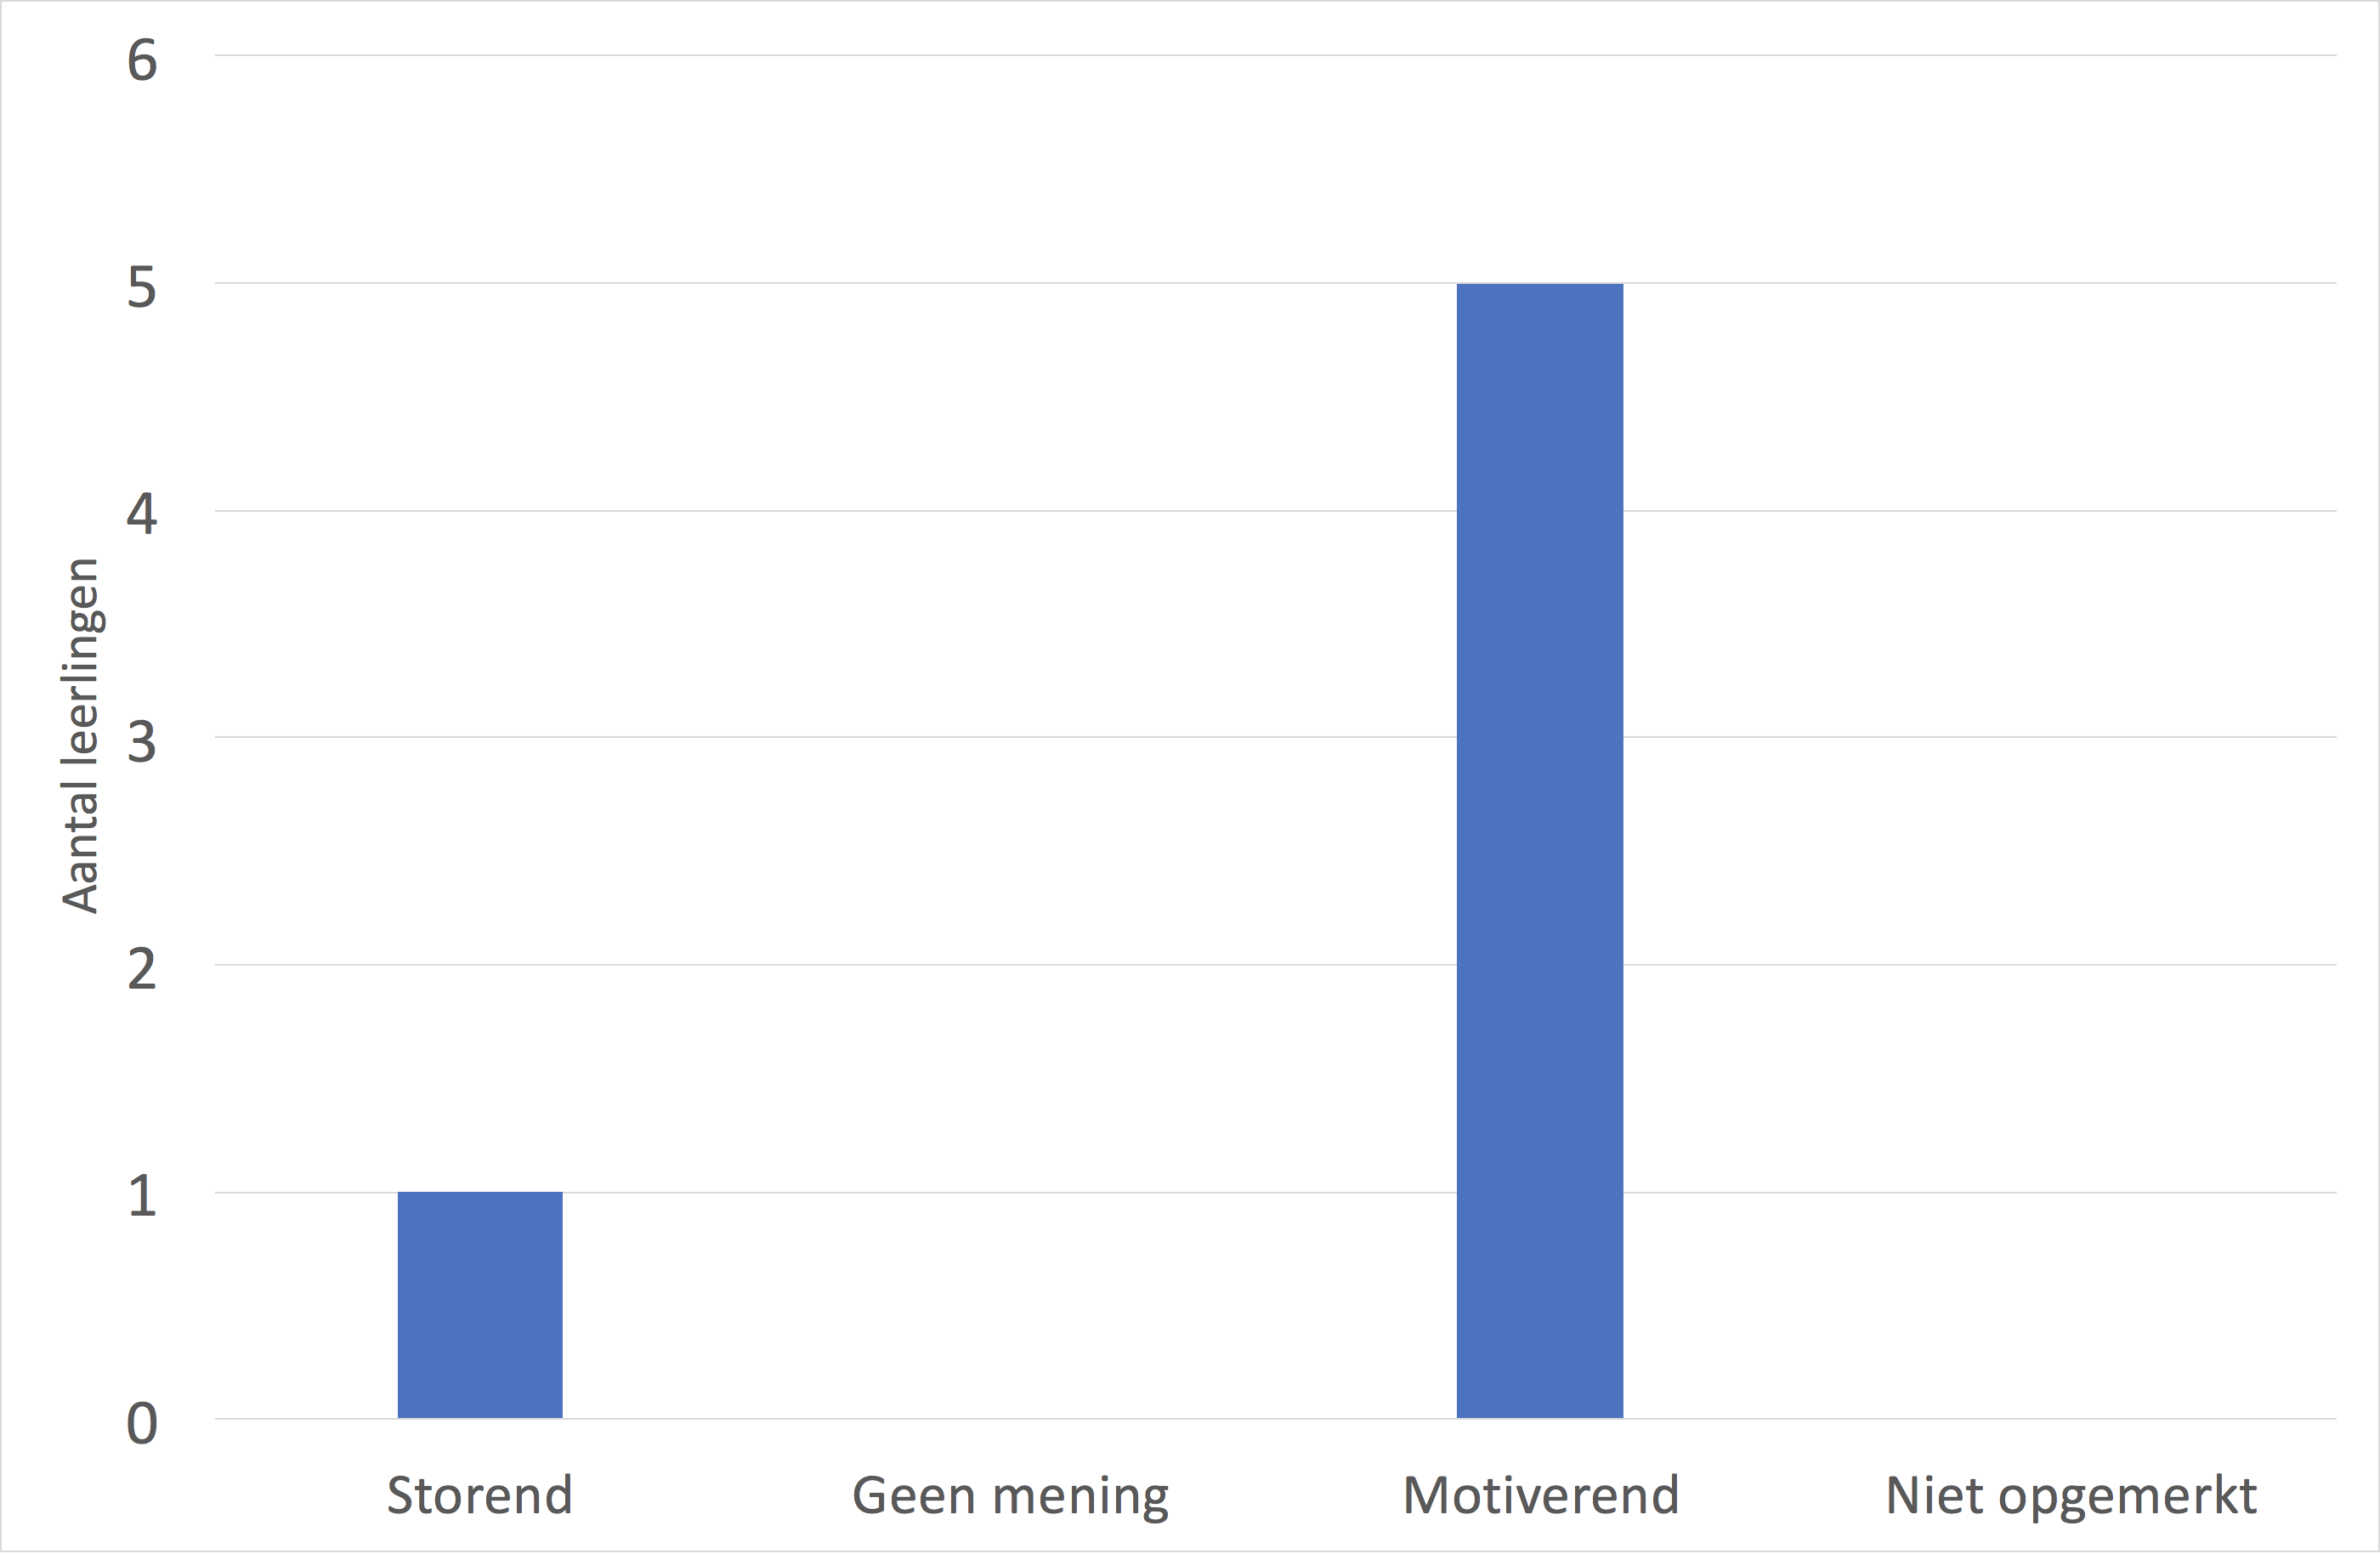
\includegraphics[width=\textwidth]{pictures/3_Achtergrondmuziek.png}
        \caption{achtergrondmuziek}
        \label{achtergrondmuziek}
    \end{subfigure}
    ~
    \begin{subfigure}[b]{0.48\textwidth}
        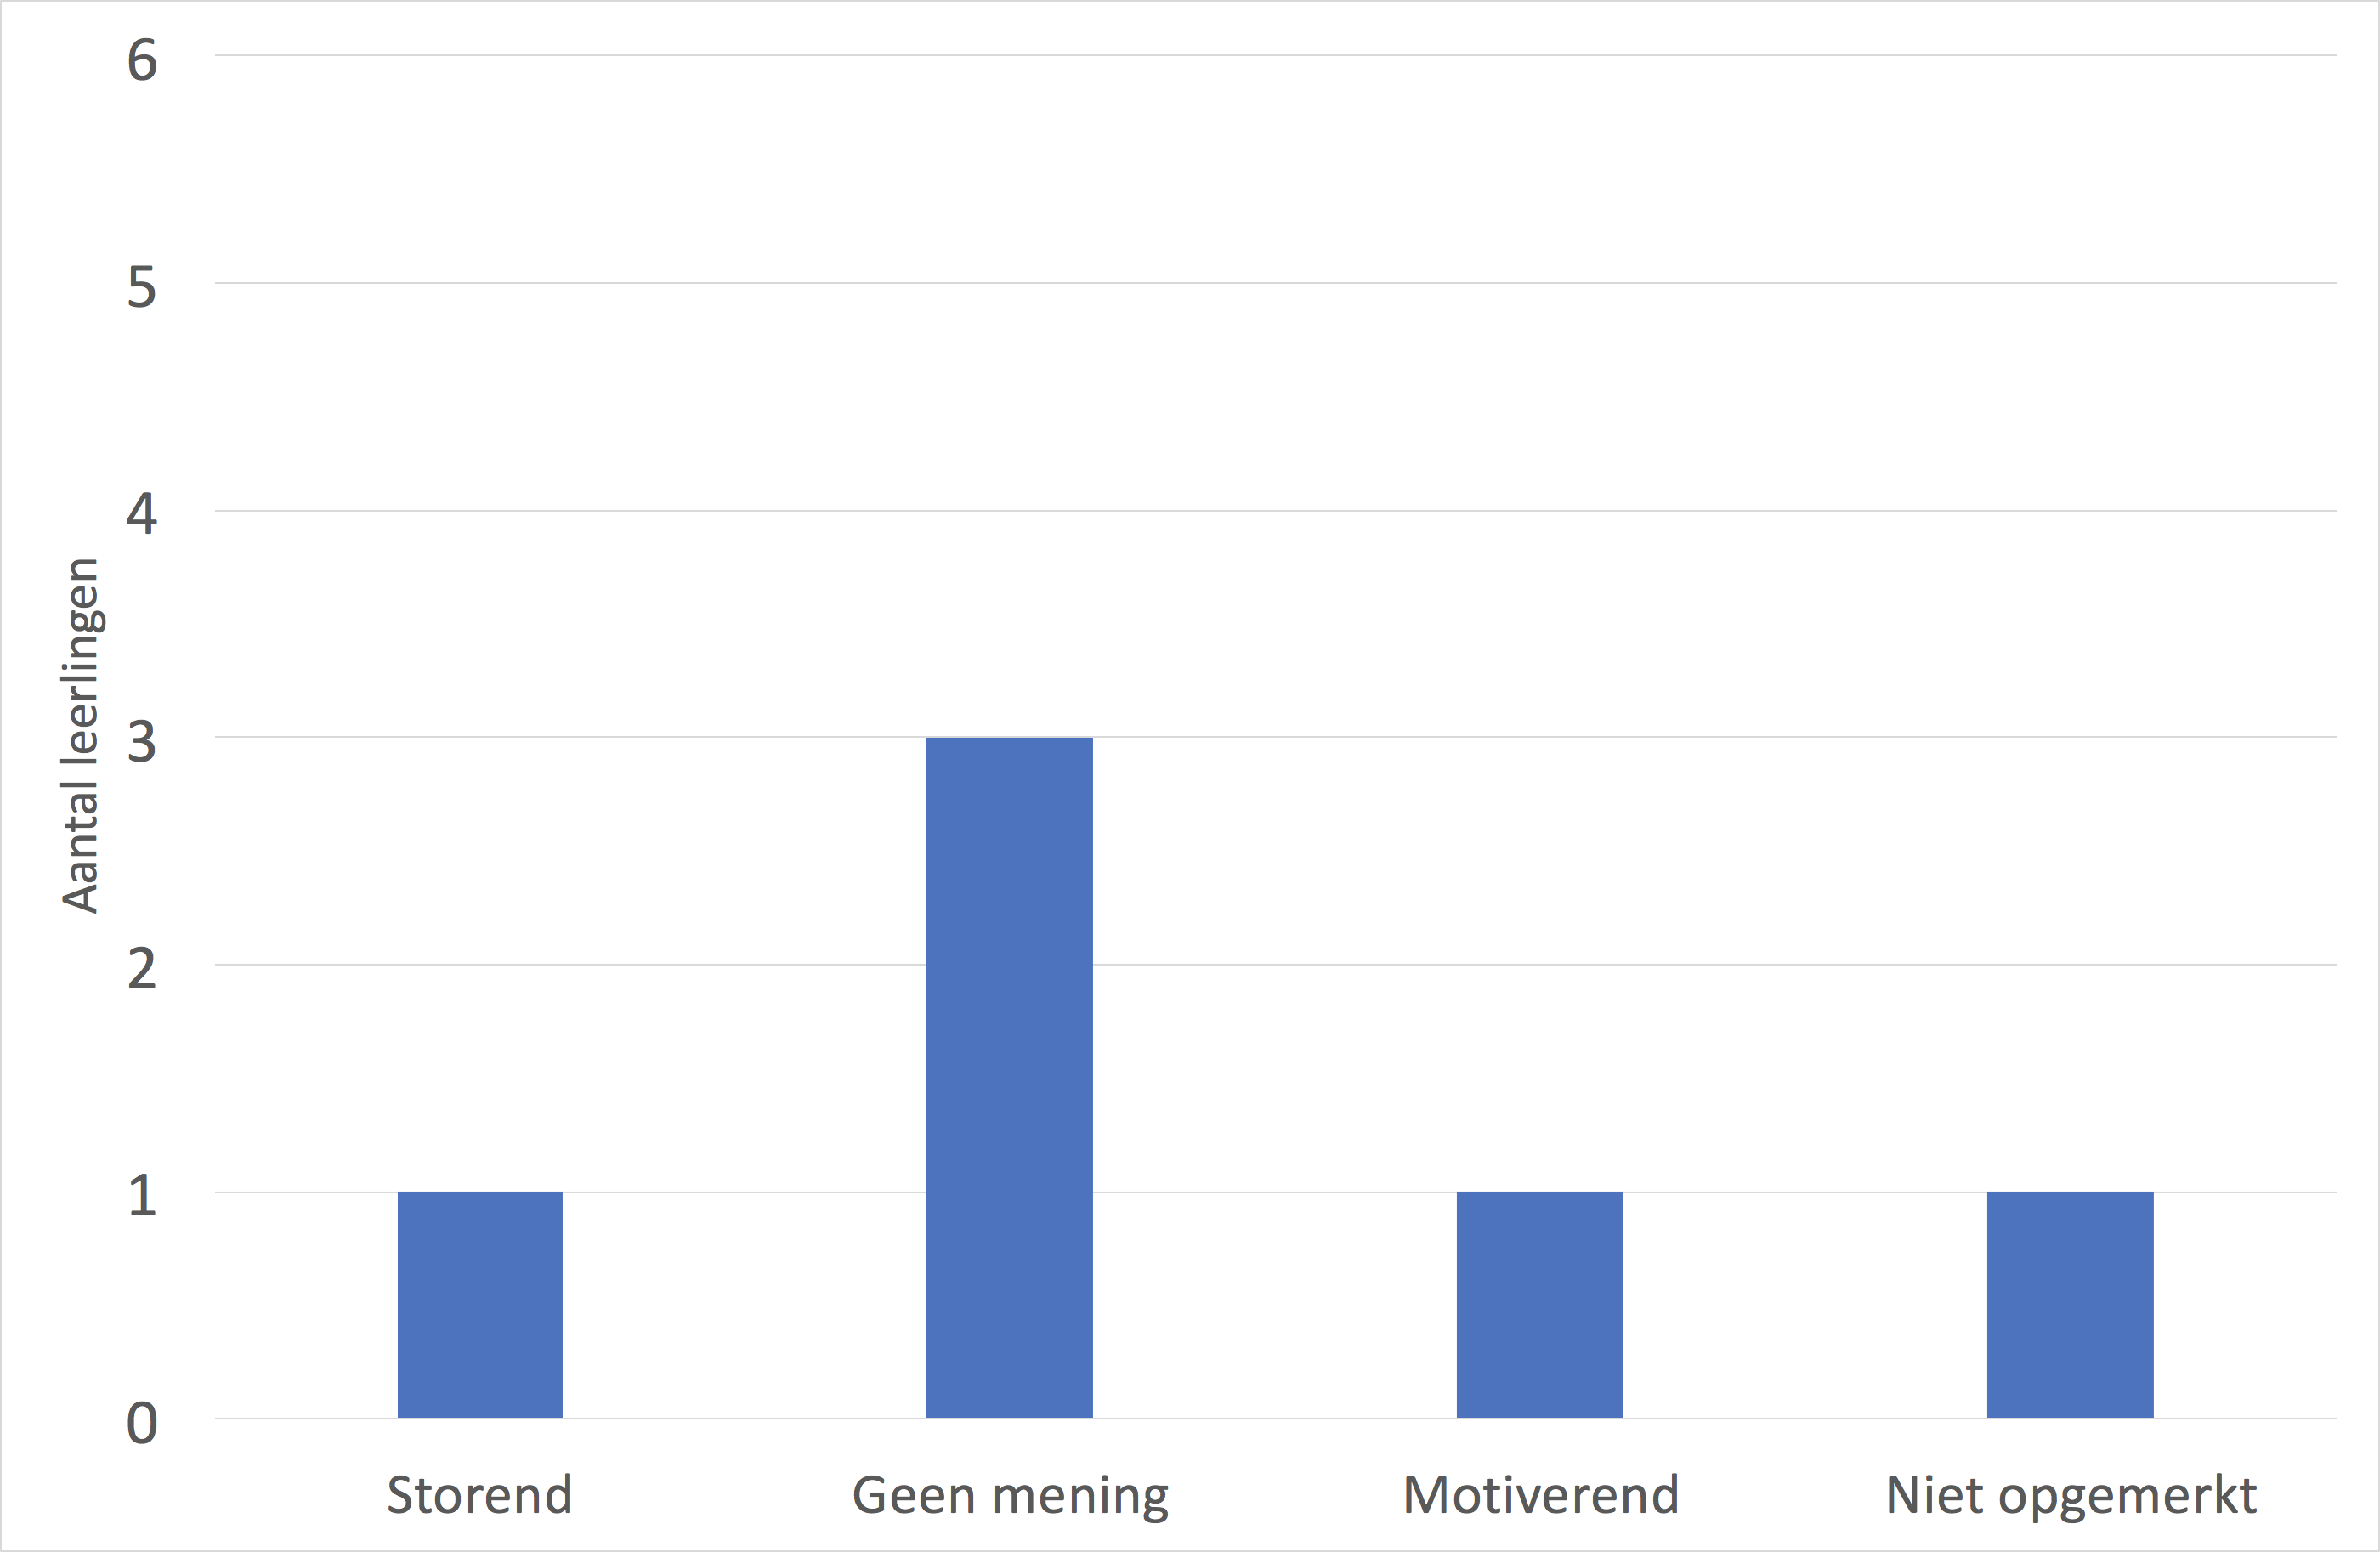
\includegraphics[width=\textwidth]{pictures/3_Spelgeluiden.png}
        \caption{spelgeluiden}
        \label{spelgeluiden}
    \end{subfigure}
    \caption{Wat vond je van de ...?}\label{geluiden}
\end{figure}

\clearpage
\section{Laatste iteratie: publicatie op Google Play Store \& App Store}
\textit{QuickMaths} kan op Android ge\"installeerd worden via \url{https://play.google.com/store/apps/details?id=cs.hciproject.quickmaths} en op iOS via \url{https://itunes.apple.com/WebObjects/MZStore.woa/wa/viewSoftware?id=1326512406&mt=8}.

	\subsection{Design keuzes}
	Tijdens een afsluitend gesprek met de leerkracht tijdens het testen van het tweede digitale prototype stelden we de vraag of het relevant zou zijn om feedback te geven aan de speler na het maken van een fout. Ze stelde voor om deze functionaliteit toe te voegen, maar zonder al te veel didactische uitleg. Bij het maken van een fout krijgt de speler te zien wat zijn fout was en wat de gepaste actie zou geweest zijn.\\\\
    Voor het \textit{``in the wild''} experiment hebben we twee verschillende gamemodi ontworpen die we met elkaar willen vergelijken. Bij het openen van de app wordt er achter de schermen bepaald welke gamemode er gebruikt wordt. De verschillende modi zijn:
    
\begin{itemize}
\item \texttt{Classic mode}: De lengte van de levels neemt logaritmisch toe en convergeert naar een maximale lengte van 20 rijen. De getallen in het speelveld worden groter volgens het level maal factor 6.
\item \texttt{Endurance mode}: De lengte van de levels neemt linearitmisch toe. De getallen in het speelveld worden wel minder snel groter: de toename is lineair volgens het level maal factor 4.
\end{itemize}
Om de resultaten van deze verschillende modi te kunnen loggen maken we gebruik van een Firebase database. Om de unieke gebruikers te kunnen identificeren maken we gebruik van een Facebook login. Spelers krijgen nog steeds de optie om te spelen zonder Facebook login, maar van deze gebruikers krijgen we geen spelstatistieken. De data die we bijhouden via logging omvat onder meer het aantal gespeelde spellen, het resultaat van het level (``gewonnen'' of ``verloren''), indien verloren welke fout gemaakt werd, welke modus gespeeld is ...\\\\
Bij deze finale versie introduceren we naast levels met sommen, verschillen en deelbaarheid ook levels met vermenigvuldigingen.
    
    \subsection{Deelnemers}
    Aan de evaluatie van deze laatste iteratie hebben in totaal $57$ personen deelgenomen. In Figuur~\ref{verdeling:man:vrouw} kan de verdeling van het aantal mannen ten opzichte van het aantal vrouwen vastgesteld worden.\\\\
    Figuur~\ref{verdeling:leeftijden} toont de verdeling van de verschillende leeftijdcategorie\"en die wij dankzij de login van Facebook kregen. Zoals vast te stellen in deze figuur, kwamen $28\%$ van de deelnemers uit onze doelgroep. Dit is vooral te wijten aan het feit dat deze doelgroep op het moment van deze evaluatie in een examenperiode zit.

\begin{figure}[h]
	\centering
	\begin{subfigure}[b]{0.45\textwidth}
    	\centering
    	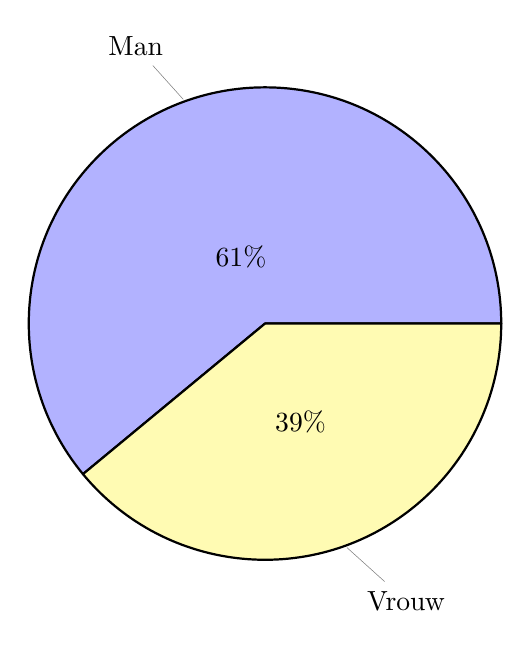
\begin{tikzpicture}
    		\pie[color={blue!30, yellow!30}, text=pin]{61/Man, 39/Vrouw}
		\end{tikzpicture}
		\caption{Verdeling Man-Vrouw}\label{verdeling:man:vrouw}
    \end{subfigure}
    ~
    \begin{subfigure}[b]{0.45\textwidth}
    	\centering
		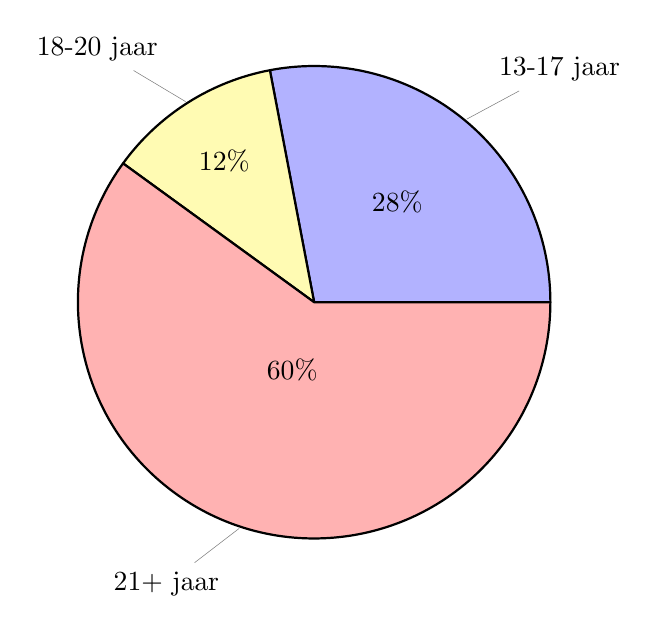
\begin{tikzpicture}
    		\pie[color={blue!30, yellow!30, red!30}, text=pin]{28/13-17 jaar, 12/18-20 jaar, 60/21+ jaar}
        \end{tikzpicture}
		\caption{Verdeling leeftijden}\label{verdeling:leeftijden}
    \end{subfigure}
    \caption{Demografische gegevens van de deelnemers}
\end{figure}

\newpage
    \subsection{Evaluatie methodes}
Bij deze kwantitatieve analyse willen we beide gamemodi vergelijken met als centrale onderzoeksvraag: 
\begin{quote} \textit{Wat is de dominante factor die de moeilijkheidsgraad van een level bepaalt: de lengte van het level of de grootte van de getallen?}
\end{quote}
We baseren ons hiervoor op de verhouding van het aantal voltooide levels tot het totaal aantal gespeelde levels.\\\\
Op basis van de gelogde gegevens kunnen we eveneens te weten komen welke modus de hoogste engagement heeft. Dit zouden we willen testen aan de hand van de hoeveelheid herkansingen van een level alvorens er wordt opgegeven (terugkeren naar hoofdmenu).

	\subsection{Resultaten}
We hebben voor drie eigenschappen een descriptieve en inferenti\"ele analyse gemaakt met de twee gamemodes als onafhankelijke veranderlijke:
\begin{itemize}
\item Failrate: de verhouding van het aantal mislukte levels tot het totaal aantal gespeelde levels
\item Hoogst behaalde level: hoogste level per speler
\item Totale speelduur: de totale speelduur per speler
\end{itemize}
Voor elke van deze eigenschappen beschrijven we een tabel met de gemiddelden en standaardafwijkingen (respectievelijk Tabel~\ref{analyse:failrates}, Tabel~\ref{analyse:levels} en Tabel~\ref{analyse:times}) en een boxplot die de verdeling duidelijk maakt (respectievelijk Figuur~\ref{failrates:gamemode}, Figuur~\ref{levels:gamemode} en Figuur~\ref{time:played:gamemode}). Voor de inferenti\"ele analyse beschrijven we voor elke eigenschap een ANOVA-tabel.

\subsubsection{Fail Rates}
Uit de ANOVA-analyse in Tabel~\ref{ANOVA-failrate} blijkt dat de gebruikte gamemode geen significante invloed heeft op de failrate (p\textgreater 0.05).
    \begin{table}[h]
		\centering
		\begin{tabular}{|lcc|}
        	\hline
			\textbf{gamemode} & \textbf{MeanFail} & \textbf{SDFail} \\
            \hline
			Classic & 42.67\% & 28.21\%  \\
			Endurance & 41.25\% & 29.01\% \\
			\hline
		\end{tabular}
		\caption{Descriptieve analyse: failrates}\label{analyse:failrates}
    \end{table}

\begin{table}[h]
\centering
\begin{tabular}{|llllll|}
\hline
 & \textbf{Df} & \textbf{Sum Sq}   & \textbf{Mean Sq} & \textbf{F value} & \textbf{Pr(\textgreater F)} \\
 \hline
\textbf{gamemode}  & 1  & 0.003    & 0.00309 & 0.038   & 0.846             \\
\textbf{Residuals} & 60 & 4.904    & 0.08173 &         &                   \\
\hline
\end{tabular}
\caption{ANOVA-analyse: failrates}
\label{ANOVA-failrate}
\end{table}

\begin{figure}[h]
	\centering
	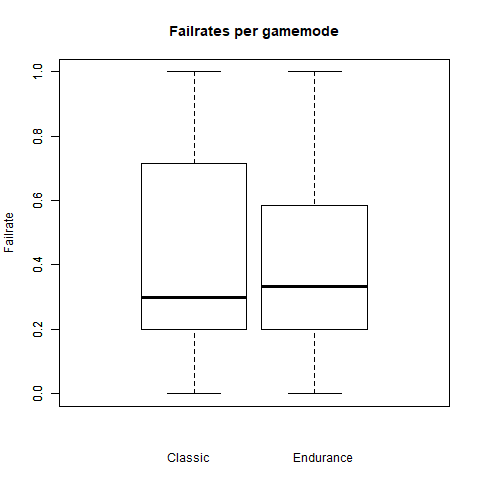
\includegraphics[width=0.5\textwidth]{pictures/Failrates.png}
    \caption{Boxplot met de failrates per gamemode per deelnemer.}
    \label{failrates:gamemode}
\end{figure}

\subsubsection{Hoogst behaalde level}
Uit de ANOVA-analyse in Tabel~\ref{ANOVA-levels} blijkt dat de gebruikte gamemode geen significante invloed heeft op het hoogst behaalde level (p\textgreater 0.05).
\begin{table}[h]
	\centering
		\begin{tabular}{|lcc|}
        	\hline
			\textbf{gamemode} & \textbf{MeanLevel} & \textbf{SDLevel} \\
            \hline
			Classic & 5.03 & 3.46  \\
			Endurance & 4.96 & 2.75 \\
			\hline
		\end{tabular}
	\caption{Descriptieve analyse: hoogst behaalde level}\label{analyse:levels}
\end{table}

\begin{table}[h]
\centering
\begin{tabular}{|llllll|}
\hline
          & \textbf{Df} & \textbf{Sum Sq}   & \textbf{Mean Sq} & \textbf{F value} & \textbf{Pr(\textgreater F)} \\
\hline
gamemode  & 1  & 0.1      & 0.072   & 0.007   & 0.933             \\
Residuals & 54 & 539.9    & 9.999   &         &                   \\
\hline
\end{tabular}
\caption{ANOVA-analyse: hoogst behaalde levels}
\label{ANOVA-levels}
\end{table}

\begin{figure}[h]
	\centering
	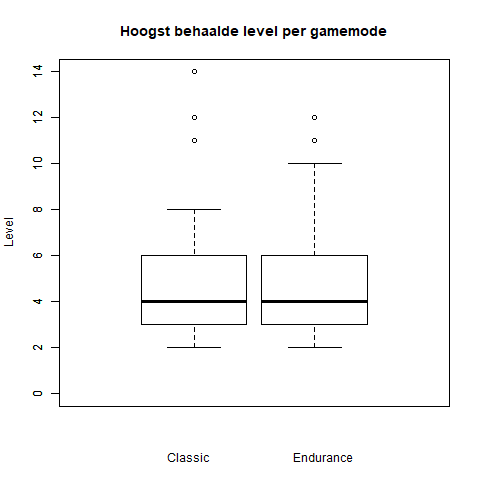
\includegraphics[width=0.5\textwidth]{pictures/Levels.png}
    \caption{Boxplot met het hoogst behaalde level per gamemode per deelnemer.}
    \label{levels:gamemode}
\end{figure}

\subsubsection{Totale speelduur}
Uit de ANOVA-analyse in Tabel~\ref{ANOVA-times} blijkt dat de gebruikte gamemode geen significante invloed heeft op de totaal gespeelde tijd (p\textgreater 0.05). Hiermee wordt ook uitgesloten dat de verschillende gamemodes significant verschillende engagement rates zouden hebben.
	\begin{table}[h]
		\centering
		\begin{tabular}{|lcc|}
        	\hline
			\textbf{gamemode} & \textbf{MeanTimes} & \textbf{SDTimes} \\
            \hline
			Classic & 370.34 & 487.43  \\
			Endurance & 250.53 & 314.65 \\
			\hline
		\end{tabular}
		\caption{Descriptieve analyse: totale speelduur}\label{analyse:times}
    \end{table}

\begin{table}[h]
\centering
\begin{tabular}{|llllll|}
\hline
          & \textbf{Df} & \textbf{Sum Sq}   & \textbf{Mean Sq} & \textbf{F value} & \textbf{Pr(\textgreater F)} \\
\hline
gamemode  & 1  & 0.1      & 0.072   & 0.007   & 0.933             \\
Residuals & 54 & 539.9    & 9.999   &         &                   \\
\hline
\end{tabular}
\caption{ANOVA-analyse: totale speelduur}
\label{ANOVA-times}
\end{table}

\begin{figure}[h]
	\centering
	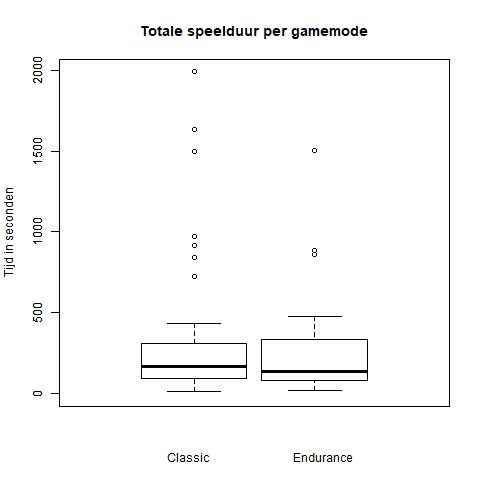
\includegraphics[width=0.5\textwidth]{pictures/TimePlayed.png}
    \caption{Boxplot met de totale speelduur per gamemode per deelnemer.}
    \label{time:played:gamemode}
\end{figure}

\subsubsection{Bespreking van de resultaten}
Uit bovenstaande resultaten blijkt duidelijk dat er geen significante verschillen zijn tussen de twee gamemodes. We kunnen dus geen uitspraak doen over de onderzoeksvraag. Een kanttekening die we hierbij willen maken is dat de hoeveelheid data uit de doelgroep zelf beperkt was. Bovendien worden de verschillen tussen beide gamemodes pas duidelijk bij het bereiken van hogere levels (vanaf level 6). In praktijk hebben de meeste spelers ongeveer dezelfde gamemode gespeeld (hoogst behaalde level is kleiner dan 6), het is bijgevolg normaal dat er geen significante verschillen werden opgemeten.

\clearpage
\section{Eindresultaat}
\noindent
Doorheen de ontwikkeling van de app hebben we gemerkt dat het niet evident is om een app te ontwikkelen die voor iedereen duidelijk is. Doorheen zowat alle iteraties werden ettelijke keren volledig tegenovergestelde meningen met ons gedeeld, waaruit we dan telkens het ``nuttige'' van het ``nutteloze'' moesten proberen te onderscheiden. Vanaf de eerste ontwerpbeslissingen werd dan ook elke finale beslissing meerdere keren gewikt en gewogen. Het uiteindelijke resultaat heeft ons het nut van meerdere iteraties, prototypes en een user-centered design bijgebracht. Als laatste punt bij onze app en het vak hebben we nog enkele bevindingen:

\begin{itemize}	
	\item Gebruikers gaan vaak te snel door tutorials en missen zo essenti\"ele informatie.
    \item Ontwerpkeuzes die triviaal leken, waren voor sommige gebruikers volledig onbegrepen.
    \item Moeilijkheid is een heel moeilijk te balanceren gegeven.
    \item Naast gebruikers, is feedback met experts ook van essenti\"eel belang.
\end{itemize}

\clearpage
\newpage
\pagenumbering{arabic}
\renewcommand*{\thepage}{Appendix p.~\arabic{page}}
\appendix
\begin{center}
	\huge{\textbf{Appendix}}
\end{center}
\section{Eerste iteratie: papieren prototype}\label{eerste:iteratie}
	\subsection{Design keuzes}
Het eerste prototype is volledig gemaakt uit papier en karton. Het dynamische, tijdsgebonden design van onze app maakt het niet makkelijk om dit op papier al te laten werken. In het uiteindelijke ontwerp hebben we gekozen voor een kartonnen gsm, met een doorschuifsysteem van papier voor ons speelveld\footnote{Foto's en afbeeldingen van het ontwerp zijn te vinden op \url{https://quickmathsblog.wordpress.com/2017/10/24/paper-prototype/}}. Hierdoor kunnen we direct de verloop van onze app volledig testen van beginscherm tot ``Game Over'' of ``Level completion".\\\\
Het ontwerp van de schermen is heel simpel gehouden. Het beginscherm laat slechts enkele simpele knoppen zien, met vooral pictogrammen.\\\\
De verschillende knoppen zijn onder andere:
\begin{itemize}
	\item Start knop, om het spel te starten,
	\item Highscores, om de beste scores weer te geven,
	\item Profiel, om de gegevens van de huidige speler te bekijken,
	\item Instellingen, om de spelinstellingen aan te passen.
\end{itemize}
Het profielscherm laat de gebruiker relevante informatie zien over:
\begin{itemize}
	\item Zichzelf
	\item ``Player status"
	\item Zijn achievements (met een knop om ze te bekijken)
	\item Top 3 beste scores
	\item Daarnaast is er de mogelijkheid om van gebruiker te wisselen.
\end{itemize}
Het speelscherm was het ingewikkeldste deel van het ontwerp. We laten het speelveld bewegen door de ``computer''-persoon van onze studie. Met ons bewegend speelveld konden we zo goed als het volledige spelverloop al testen. Het ontwerp hiervan is heel simpel. Eerst laten we de vraag zien waarover de speler moet gaan nadenken. Na een countdown tonen we het effectieve speelveld.\\\\
Afhankelijk van hoe goed de speler het doet, komt er een ``Level klaar''- of ``Game over''-scherm. Het “Level klaar”-scherm laat de gebruiker toe om verder te gaan naar het volgende (moeilijkere) level, of om terug te keren naar het beginscherm. ``Game over'' laat toe om het level opnieuw te proberen of om terug te keren naar het beginscherm.
    
	\subsection{Deelnemers}
De doelgroep van onze applicatie zijn de leerlingen van de eerste graad middelbare school. Hiervoor hebben wij contact opgenomen met het Heilig Hartinstituut te Heverlee\footnote{\url{https://www.hhh.be/home}}. Aangezien het ons wat moeite gekost heeft om deze te bereiken en afspraken te maken, hebben we voor de eerste iteratie een drietal studenten op het departement Computerwetenschappen gevraagd om deel te nemen aan deze gebruikersstudie.
    
    \subsection{Evaluatie methodes}
Voor de eerste evaluatie van dit papieren prototype hebben we gebruik gemaakt van een think-aloud study. We hebben met deze eerste evaluatie al vroeg in het ontwerpproces enkele tekortkomingen geïdentificeerd. Dit was waardevol vermits deze tekortkomingen reeds duidelijk werden op basis van het papieren prototype. Er werd rekening gehouden met de opmerkingen bij het ontwerp van het eerste digitale prototype. De deelnemers werden gevraagd om een level te spelen tot voltooiing, en om vervolgens hun profielpagina te bekijken.

	\subsection{Resultaten}
De voornaamste bevindingen worden beschreven in Tabel~\ref{Issues-PP}.
    \begin{table}[H]
		\centering
		\begin{tabular}{|l l l l|}
        	\hline
			& \textbf{Begin van spel} & \textbf{Waar antwoord kiezen} & \textbf{Overblijvende tijd} \\
            \hline
			Speler A & Pas duidelijk na uitleg & Pas duidelijk na uitleg & Geen problemen\\
			Speler B & Meteen duidelijk & Duidelijk & Verwarrend\\
			Speler C & Meteen duidelijk & Duidelijk & Verwarrend\\
			\hline
		\end{tabular}
		\caption{Usability issues van papieren prototype}\label{Issues-PP}
    \end{table}
\noindent
Speler A start het spel, de opgave en countdown volgen elkaar op en het speelveld verschijnt. Speler~A overschouwt het speelveld en begint cellen aan te duiden, de speler raakt verward en geeft na een tiental seconden op. De observer geeft een tip en verwijst naar de roodgekleurde speelbalk. De speler was vergeten dat $0$ deelbaar is door $7$. Na deze tips is speler A erin geslaagd om het level te voltooien. Vervolgens vindt de speler zijn weg naar de profielpagina via het home scherm, en vindt hij zijn status: ``Speed Junky''. Om de verwarring bij de start van het spel op te lossen, zal er in het vervolg bij de start van het spel een lege lijn in de speelbalk verschijnen die meteen doorgeschoven wordt met de eerste ``echte lijn''.\\\\
Speler B weet meteen waar de inputs geregistreerd worden (roze balk). De speler doorloopt de eerste lijnen, maar maakt vervolgens een fout door een antwoord aan te duiden op een lijn waar geen juiste antwoorden zijn. Deze verwarring zou verholpen kunnen worden door deze mechanic in de korte tutorial uit te leggen. Het game-over scherm wordt getoond en de speler vindt zijn weg naar de profielpagina. De speler had wel nog een opmerking dat het tijdens het spel niet duidelijk is hoeveel tijd er is om een antwoord te geven. In het digitale prototype zullen we de pauze knop (onderaan het scherm) gebruiken om de overblijvende tijd per lijn te tonen als een balk die gevuld wordt van links naar rechts.\\\\
Speler C begint aan het spel en merkt de speelbalk meteen op. Halfweg het level slaagt de speler er niet in om op tijd een antwoord te geven, en eindigt het spel. De speler verwijst net als speler B naar een nood om de overblijvende tijd te kunnen zien. De speler vindt eveneens makkelijk de weg naar de profielpagina om de player status te bekijken.\\\\
Tijdens de study kwamen we samen tot inzicht dat er op alle schermen buiten het home screen er nog een ``Keer terug''-knop ontbreekt. We brengen deze feedback in rekening bij de ontwikkeling van het digitale prototype.

\newpage
\section{Tweede iteratie: eerste digitale prototype}\label{tweede:iteratie}
	\subsection{Design keuzes}
Het digitale prototype is qua ontwerp zeer gelijkend op het papieren prototype\footnote{Foto's en afbeeldingen van deze versie te vinden op: \url{https://quickmathsblog.wordpress.com/2017/11/13/digitale-prototype-eerste-versie/}}.\\\\
Bij het opstarten van het spel wordt de speler begroet door het ``beginscherm''. Na te drukken op de startknop, krijgt de gebruiker een korte tutorial. In deze tutorial krijgt de gebruiker in een viertal afbeeldingen uitgelegd hoe het spel werkt en wat hij precies moet doen. Hierna kan hij verder gaan naar het menu.\\\\
Het menu geeft de gebruiker vier toetsen om te selecteren: ``Play'', ``Highscores'', ``Profile'' en ``Settings''.
Twee van de knoppen staan centraal en zijn anders gekleurd, hiermee trekken we de aandacht naar de belangrijkste features van de app.\\\\
Bij de start van een level worden de opgave, een countdown en een voorbeeld van hoe het spel werkt getoond. Na de countdown begint het spel. Tijdens het spel weergeven we enkele belangrijke elementen op het scherm:
\begin{itemize}
	\item Links bovenaan: de opgave,
	\item Rechts bovenaan: het resterend aantal lijnen en het huidige level,
	\item Midden op scherm: de volgende rijen. Deze zijn lichtjes geblurred om de aandacht meer te vestigen op de speelbalk, onderaan.
	\item Onderaan: de speelbalk met de deadline onderaan. Deze deadline geeft de resterende tijd voor deze lijn in de speelbalk aan.
\end{itemize}
In de loop van het spel worden er steeds nieuwe lijnen aan de gebruiker voorgeschoteld. De knoppen worden gehighlight aan de hand van de input. Indien de gebruiker het juiste antwoord heeft aangeduid (of niets, als er geen juiste oplossing was), dan gaat het spel verder en krijgt hij een volgende lijn te zien. Zolang de deadline van deze lijn niet verstreken is, kan hij zijn antwoord nog aanpassen. Indien het fout ging, tonen we het ``Game Over'' scherm.\\\\
Het ``Game Over'' scherm laat toe om terug te keren naar het menu of het huidige level terug te proberen met een andere opgave. Is de gebruiker geslaagd voor alle lijnen van het level, dan gaat hij naar het ``Level voltooid'' scherm. Hierin krijgt hij de keuze om verder te gaan naar het volgende level of terug te keren naar menu. Bij het terugkeren wordt de gebruiker gewaarschuwd dat hij zijn huidige vooruitgang zal verliezen.\\\\
In het digitale prototype zijn er nog geen andere features ondersteund. Het profiel bestaat uit een dummy scherm dat een mogelijke indeling geeft voor de latere implementaties.
    
	\subsection{Deelnemers}
Aan de evaluatie van deze iteratie hebben vier leerlingen en \'e\'en leerkracht wiskunde van het Heilig Hartinstituut te Heverlee deelgenomen. In Tabel~\ref{demografie:tweede:iteratie} kunnen de demografische gegevens over de deelnemers van deze gebruikersstudie van de tweede iteratie teruggevonden worden.
	
    \begin{table}[H]
		\centering
		\begin{tabular}{|lcc|}
        	\hline
			& \textbf{leeftijd} & \textbf{studierichting} \\
            \hline
			leerling 1 & 12 & Latijn \\
			leerling 2 & 12 & Latijn \\
			leerling 3 & 11 & Latijn \\
			leerling 4 & 12 & Latijn \\
			leerkracht & 43 & \\
			\hline
		\end{tabular}
		\caption{Demografie deelnemers tweede iteratie}\label{demografie:tweede:iteratie}
    \end{table}
    
    \subsection{Evaluatie methodes}
Voor de evaluatie van dit eerste digitale prototype doen we een think-aloud study met deelnemers uit onze doelgroep. De deelnemers worden gevraagd om de eerste twee levels te voltooien, en om vervolgens hun profielpagina te bekijken. Het think-aloud aspect van deze studie is vooral interessant wanneer de gebruiker een fout maakt of wanneer de gebruiker op verkenning gaat in de app. Tijdens het spelen van het spel zelf, ondervinden ze dat het erg moeilijk is om tegelijkertijd luidop te denken en de oefeningen op te lossen.

	\subsection{Resultaten}
We vroegen aan elke deelnemer om level 1 te voltooien. Zodra dit lukte, werden ze gevraagd om verder te spelen totdat ze level 3 voltooid hadden. Mits enkele tussenkomsten van de moderator, slaagde iedereen er in om deze taken binnen aanvaardbare tijd te voltooien.
\begin{sidewaystable}
\begin{table}[H]
\centering
\def\arraystretch{1.2}
\begin{tabular}{m{2cm}|m{1.5cm}|m{1.5cm}|m{4cm}|m{4cm}|m{4.5cm}}
& \textbf{Leeftijd} & \textbf{Geslacht} & \textbf{Start van het spel } & \textbf{Lege vakjes} & \textbf{Rijen zonder oplossing}\\ \hline
Persoon 1 & 12 & V & Ik snapte niet direct waar dat ik op moest klikken. & Verwarring over selecteren: juist of fout? & Lichte verwarring, maar geen probleem \\\hline 
Persoon 2 & 12 & M & De tijd en meerdere keuze vragen & Geen probleem & Wilde steeds iets selecteren, zelfs foute oplossingen \\\hline 
Persoon 3 & 11 & M & Ik wist niet hoe ik het moest doen. & Twijfelde lichtjes, maar maakte geen fout & Geen probleem \\\hline 
Persoon 4 & 12 & M & Ik wist niet waar ik moest drukken & Geen probleem & Geen probleem\\ \hline
Persoon 5 & 43 & V & Verwarring, geen idee wat te doen na countdown. & Geen probleem & Geen probleem\\ \hline 

\multicolumn{3}{c|}{\multirow{4}{*}{Mogelijke oplossingen:} }  & - Intro moet minder druk worden. & Geen lege vakjes. & Maakt inherent deel uit van de uitdaging. \\
\multicolumn{3}{c|}{} & - Countdown moet opvallender. & Vermelden in tutorial. & Valstrik, extra uitdaging. \\
\multicolumn{3}{c|}{} & - Meer contrast tussen speelveld en -balk. & & \\
\multicolumn{3}{c|}{} & - Statische tutorial maakt al veel duidelijk. & & \\ \hline
\multicolumn{3}{c|}{Algemene opmerking: }  & \multicolumn{2}{c}{Er werd geen tutorial getoond aan de proefpersonen.} & \\ \hline
\end{tabular}

\caption{Resultaten think-aloud study paper prototype 1}\label{TA:S1}
\end{table}
\end{sidewaystable}\\\\
Tijdens het uitvoeren van deze taken, stelden zich enkele problemen. Deze problemen worden beschreven en geëvalueerd, inclusief een mogelijke oplossing. Hiervoor verwijzen we naar onderstaande tabel. In de volgende iteratie(s) zullen deze problemen geadresseerd worden. We proberen daarna opnieuw testen te doen met onze doelgroep.\\\\
Als laatste punt geven we nog enkele opmerkelijke resultaten mee van onze enquête:
\begin{itemize}
\item E\'en van de testpersonen bleek licht gefrustreerd na onze testen. Opmerkelijk was dat deze persoon wel wilde meewerken in verdere testen.
\item De moeilijkheid van ons spel bleek voor iedereen ook anders: twee personen vonden het makkelijk tot gemiddeld, twee personen vonden het heel moeilijk.
\item De leerlingen wilden het spel gebruiken om vlotter te worden in basis hoofdrekenen.
\item Alle deelnemers willen de app meerdere keren per week spelen.
\end{itemize}

\newpage
\section{Dataparser - Code}\label{python:code}
	\pythonexternal{input/parser.py}

\newpage
\section{Analyse - Code}\label{r:code}
    \rexternal{input/QMMarkdown.Rmd}

\end{document}
